\chapter{拟牛顿法}
\label{chap:quasi-newton}

假设目标有$n=10^4$个变量，算一次梯度只需几毫秒。第~\ref{chap:second-order-methods}章的Newton法收敛很快，但它每一步都要形成Hessian，保存约$5\times10^7$个不同的元素，再做一次约$3\times10^{11}$次运算的分解。第~\ref{chap:first-order-methods}章的梯度下降每步只需要梯度，可是在狭长的山谷里它不断来回折返，因为它完全不知道地形朝哪个方向弯得厉害。

这两者之间有一个常被浪费的信息来源。迭代走了一步之后，我们手里有相邻两点的梯度，两个梯度的差反映了这一段路上地形的弯曲。这件事不需要额外的计算，只要把数字留下来。

本章研究怎样把这些“免费”的曲率测量攒成一个可用的矩阵。第~\ref{sec:qn-secant}节写出测量给出的条件，并说明为什么单靠它定不出矩阵。第~\ref{sec:qn-dfp-bfgs}节用两个秩一项做修正，得到DFP和BFGS两种更新，重点在怎样保持矩阵正定。

第~\ref{sec:qn-sr1}节只用一个秩一项，它能记住负曲率，代价是失去正定性。第~\ref{sec:qn-lbfgs}节处理连$n\times n$矩阵都存不下的情形，只保留最近几次测量。第~\ref{sec:qn-convergence}节在同一套条件下逐个核对这些方法能保证什么，并按相同精度比较计算成本。

全章用同一个二维目标做手算：
\begin{equation}
 f(\bm{x})=x_1^2+4x_2^2,\qquad \bm{x}^{(0)}=(4,1)^\top.
 \label{eq:qn-running-example}
\end{equation}
它的Hessian是$\bm{A}=\operatorname{diag}(2,8)$，最优解是原点。算法并不知道$\bm{A}$，它只能在迭代点上读取梯度$\nabla f(\bm{x})=\bm{A}\bm{x}$。

\section{割线条件}
\label{sec:qn-secant}

不计算Hessian，单凭已经读到的梯度，能知道多少曲率？答案是一条线性方程组，它精确地说出了一次测量包含的信息，也说明了这些信息还远远不够。

\paragraph{用近似矩阵代替Hessian}
Newton法在当前点$\bm{x}^{(t)}$处用二次模型近似目标。把模型里的Hessian换成一个对称矩阵$\bm{B}^{(t)}$，模型变成
\begin{equation}
 m^{(t)}(\bm{p})=f(\bm{x}^{(t)})+\langle\bm{g}^{(t)},\bm{p}\rangle+\frac12\bm{p}^\top\bm{B}^{(t)}\bm{p}.
 \label{eq:qn-model}
\end{equation}
当$\bm{B}^{(t)}$正定时，模型是严格凸的，令它的梯度$\bm{g}^{(t)}+\bm{B}^{(t)}\bm{p}$为零，得到唯一极小点
\begin{equation}
 \bm{d}^{(t)}=-\bm{W}^{(t)}\bm{g}^{(t)},\qquad\bm{W}^{(t)}=\bigl(\bm{B}^{(t)}\bigr)^{-1}.
 \label{eq:qn-direction}
\end{equation}
这里$\bm{B}^{(t)}$叫曲率近似，$\bm{W}^{(t)}$叫逆曲率近似。全卷$\bm{H}^{(t)}$专指真实Hessian，所以逆近似用$\bm{W}$表示。下面只需要回答一件事：这两个矩阵从哪里来。

\paragraph{一维情形：割线}
先看只有一个变量的目标。设$f(x)=\tfrac14x^4+\tfrac12x^2$，梯度$g(x)=x^3+x$，已经走过$x^{(0)}=1$和$x^{(1)}=0.5$，读到
\[
 g(x^{(0)})=2,\qquad g(x^{(1)})=0.625.
\]
过这两点作$g$的割线，斜率是
\[
 b=\frac{g(x^{(1)})-g(x^{(0)})}{x^{(1)}-x^{(0)}}=\frac{0.625-2}{0.5-1}=2.75.
\]

这个斜率介于两端的真实二阶导数$f''(0.5)=1.75$与$f''(1)=4$之间。由微积分基本定理，它正好是$f''$在这一段上的平均值。把$b$当作曲率，下一个点就是割线与横轴的交点：
\[
 x^{(2)}=x^{(1)}-\frac{g(x^{(1)})}{b}=0.5-\frac{0.625}{2.75}\approx0.273.
\]
图~\ref{fig:qn-secant-1d}画出了这一步。割线不如切线精确，却不需要二阶导数，只用两次已经算过的梯度。

\begin{BookInlineFigure}
  \centering
  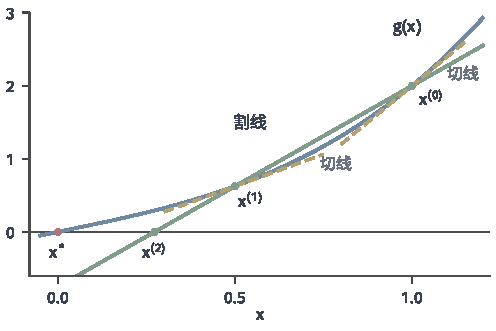
\includegraphics[width=84mm]{figures/05-optimization/02-smooth-optimization/matplotlib/qn-secant-1d/figure.pdf}
  \caption{一维的割线步。蓝线是$f(x)=\tfrac14x^4+\tfrac12x^2$的梯度$g(x)=x^3+x$。绿线是过$x^{(0)}=1$、$x^{(1)}=0.5$两点的割线，斜率$2.75$是$f''$在这一段的平均值；两条黄色虚线是两端的切线，斜率分别为$4$和$1.75$。割线与横轴的交点给出下一个迭代点$x^{(2)}\approx0.273$，红点是最优解。}
  \label{fig:qn-secant-1d}
\end{BookInlineFigure}

\paragraph{高维情形：梯度差是平均曲率作用于位移}
高维时除法做不了，但关系仍在。记位移与梯度差分别为
\begin{equation}
 \bm{s}^{(t)}=\bm{x}^{(t+1)}-\bm{x}^{(t)},\qquad\bm{y}^{(t)}=\bm{g}^{(t+1)}-\bm{g}^{(t)}.
 \label{eq:qn-s-y}
\end{equation}
沿线段$\bm{x}^{(t)}+\tau\bm{s}^{(t)}$（$\tau\in[0,1]$）对梯度用微积分基本定理，得到
\begin{equation}
 \bm{y}^{(t)}=\bar{\bm{H}}^{(t)}\bm{s}^{(t)},\qquad
 \bar{\bm{H}}^{(t)}=\int_0^1\nabla^2f\bigl(\bm{x}^{(t)}+\tau\bm{s}^{(t)}\bigr)\,\mathrm{d}\tau.
 \label{eq:qn-average-hessian}
\end{equation}
所以$\bm{y}^{(t)}$是这一段路上的平均Hessian作用在位移上的结果。对二次目标，Hessian是常数$\bm{A}$，等式成为精确的$\bm{y}^{(t)}=\bm{A}\bm{s}^{(t)}$。

可以把每一步想成一次路试。车沿某条路开过去，记下坡度的变化，就知道这条路上地形弯得多厉害。对应关系是：路线对应$\bm{s}^{(t)}$，坡度变化对应$\bm{y}^{(t)}$，弯曲程度对应$\bar{\bm{H}}^{(t)}$在这个方向上的作用。

这个类比有两处要小心。一次路试只告诉我们沿路线方向的信息，与路线垂直的方向几乎没有测量；地形不是二次的时候，旧路试测到的曲率会随着位置改变而过时。

既然模型要代表目标在下一个点的局部形状，自然要求新的矩阵重现最新的测量。

\begin{definition}[割线条件]
\label{def:qn-secant}
给定$\bm{s}^{(t)}$与$\bm{y}^{(t)}$，称对称矩阵$\bm{B}^{(t+1)}$满足\term{割线条件}（secant condition），如果
\begin{equation}
 \bm{B}^{(t+1)}\bm{s}^{(t)}=\bm{y}^{(t)}.
 \label{eq:qn-secant}
\end{equation}
用逆曲率近似$\bm{W}^{(t+1)}$表示时，条件写成
\begin{equation}
 \bm{W}^{(t+1)}\bm{y}^{(t)}=\bm{s}^{(t)}.
 \label{eq:qn-secant-inverse}
\end{equation}
\end{definition}

割线条件有一个几何含义。以$\bm{x}^{(t+1)}$为中心的模型在新点的梯度是$\bm{g}^{(t+1)}$，在旧点（$\bm{p}=-\bm{s}^{(t)}$）的梯度是
\[
 \bm{g}^{(t+1)}-\bm{B}^{(t+1)}\bm{s}^{(t)}=\bm{g}^{(t+1)}-\bm{y}^{(t)}=\bm{g}^{(t)}.
\]
也就是说，模型在新旧两点的梯度都与目标一致。使用满足割线条件的矩阵，并按这种方式选择方向的方法统称\term{拟牛顿法}（quasi-Newton method）。

下面用贯穿例算出第一组测量。取$\bm{W}^{(0)}=\bm{I}$，第一步就是负梯度方向。在二次目标上，沿方向$\bm{d}$的精确线搜索步长是
\[
 \alpha=\frac{-\langle\bm{g},\bm{d}\rangle}{\bm{d}^\top\bm{A}\bm{d}}.
\]
代入第一轮的数据，得到
\[
 \bm{g}^{(0)}=(8,8)^\top,\qquad\bm{d}^{(0)}=(-8,-8)^\top,\qquad\alpha^{(0)}=\frac{128}{640}=\frac15.
\]

走完这一步，得到新的点和梯度：
\[
 \bm{x}^{(1)}=(2.4,-0.6)^\top,\qquad\bm{g}^{(1)}=(4.8,-4.8)^\top.
\]
位移和梯度差是
\begin{equation}
 \bm{s}^{(0)}=(-1.6,-1.6)^\top,\qquad\bm{y}^{(0)}=(-3.2,-12.8)^\top.
 \label{eq:qn-running-pair}
\end{equation}

\paragraph{一条割线条件定不出矩阵}
割线条件有$n$个方程，对称矩阵有$n(n+1)/2$个自由元素，还差$n(n-1)/2$个条件。$n=1$时恰好相等，这正是一维割线法没有选择余地的原因。$n$一大，缺口迅速变大。

图~\ref{fig:qn-secant-unknowns}说明缺的是哪些信息。把$\bm{s}$单位化后作为第一个基向量。$\bm{B}\bm{s}=\bm{y}$确定了矩阵的第一列，对称性再确定第一行，其余$(n-1)\times(n-1)$的对称块完全自由。换句话说，矩阵在与$\bm{s}$正交的子空间内怎样弯曲，这次路试没有提供任何信息。

\begin{BookInlineFigure}
  \centering
  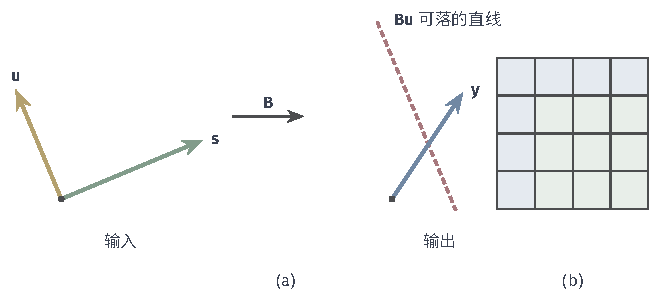
\includegraphics[width=110mm]{figures/05-optimization/02-smooth-optimization/tikz/qn-secant-unknowns/figure.pdf}
  \caption{割线条件确定了矩阵的哪些部分。(a)$n=2$时，$\bm{B}$把$\bm{s}$送到已知的$\bm{y}$；对另一个方向$\bm{u}$，对称性只给出$\langle\bm{Bu},\bm{s}\rangle=\langle\bm{u},\bm{y}\rangle$，所以$\bm{Bu}$只知道落在红色虚线上。(b)$n=4$时，在以$\bm{s}$为第一个基向量的正交基下，蓝色的第一行第一列由割线条件和对称性确定，绿色的$3\times3$对称块的$6$个元素仍然自由。}
  \label{fig:qn-secant-unknowns}
\end{BookInlineFigure}

用贯穿例看得更具体。设$\bm{B}=\begin{bmatrix}a&b\\b&c\end{bmatrix}$，把式~\eqref{eq:qn-running-pair}代入割线条件，两个方程约去公因子后是
\[
 a+b=2,\qquad b+c=8.
\]
三个未知数、两个方程，还剩一个自由参数：
\begin{equation}
 \bm{B}(a)=\begin{bmatrix}a&2-a\\2-a&6+a\end{bmatrix},\qquad
 \det\bm{B}(a)=10a-4.
 \label{eq:qn-secant-family}
\end{equation}
真实Hessian是其中$a=2$的成员，但算法无从知道。

族中不同成员给出的方向也不同。若第一步取较短的步长$\alpha^{(0)}=1/8$，位移与梯度差只差一个倍数，方程不变，于是仍是族~\eqref{eq:qn-secant-family}。此时$\bm{x}^{(1)}=(3,0)^\top$，$\bm{g}^{(1)}=(6,0)^\top$，方向$-\bm{B}(a)^{-1}\bm{g}^{(1)}$的计算结果是
\[
 \begin{aligned}
 a=0.9:&\quad(-8.28,\ 1.32)^\top,\\
 a=2:&\quad(-3,\ 0)^\top,\\
 a=5:&\quad(-1.435,\ -0.391)^\top.
 \end{aligned}
\]

只有$a=2$的方向一步落到最优解。图~\ref{fig:qn-secant-family}(a)把这些模型画在一起：它们在$\bm{x}^{(0)}$处都与同一条红色切线相切，这是割线条件保证的，在别的地方却差别很大，极小点也各不相同。

\begin{BookInlineFigure}
  \centering
  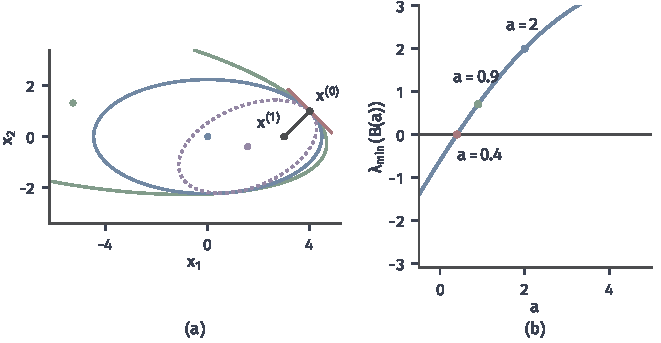
\includegraphics[width=112mm]{figures/05-optimization/02-smooth-optimization/matplotlib/qn-secant-family/figure.pdf}
  \caption{满足同一割线条件的矩阵族~\eqref{eq:qn-secant-family}。(a)从$\bm{x}^{(0)}=(4,1)$走到$\bm{x}^{(1)}=(3,0)$后，$a=0.9$（绿）、$a=2$（蓝）、$a=5$（紫，点线）三个模型过$\bm{x}^{(0)}$的等值线，它们在$\bm{x}^{(0)}$处有同一条切线（红），同色小点是各模型的极小点。(b)$\bm{B}(a)$的最小特征值，$a>0.4$时为正。}
  \label{fig:qn-secant-family}
\end{BookInlineFigure}

\paragraph{还要补充什么要求}
既然割线条件不够，就要额外规定想要什么样的矩阵。后面各种方法的区别，就在这些补充要求上。

第一是\textbf{对称}。Hessian对称，近似矩阵也应该对称，这已经写进了定义。

第二是\textbf{低秩修正}：$\bm{B}^{(t+1)}$与$\bm{B}^{(t)}$只差一个秩很低的矩阵。这样做既保留了以前路试积累的信息，也使更新只花$O(n^2)$次运算。它还能配合逆矩阵的公式，直接更新$\bm{W}$，于是根本不用解线性方程。

第三是\textbf{曲率性质}。我们希望$\bm{B}^{(t+1)}$正定，这样方向~\eqref{eq:qn-direction}才是模型的极小点。但正定性对测量数据有要求。用$\bm{s}^{(t)}$与割线条件~\eqref{eq:qn-secant}作内积，得到
\begin{equation}
 \bigl(\bm{s}^{(t)}\bigr)^\top\bm{B}^{(t+1)}\bm{s}^{(t)}=\langle\bm{s}^{(t)},\bm{y}^{(t)}\rangle.
 \label{eq:qn-curvature-identity}
\end{equation}
左边在$\bm{B}^{(t+1)}\succ\bm{0}$且$\bm{s}^{(t)}\neq\bm{0}$时为正，所以必须有
\begin{equation}
 \langle\bm{s}^{(t)},\bm{y}^{(t)}\rangle>0.
 \label{eq:qn-curvature-condition}
\end{equation}
这个不等式称为\term{曲率条件}（curvature condition）。它的含义是：沿刚走过的路，平均来看地形向上弯。

曲率条件确实可能不成立。取不定的二次目标，其Hessian为$\operatorname{diag}(2,-1)$，$\bm{s}=(1,2)^\top$，则
\[
 \bm{y}=(2,-2)^\top,\qquad\langle\bm{s},\bm{y}\rangle=2-4=-2<0.
\]
这时任何满足割线条件的矩阵都不可能正定。曲率条件是必要条件，第~\ref{sec:qn-dfp-bfgs}节将说明，配合恰当的更新，它也是充分的。

\paragraph{接入线搜索}
得到$\bm{W}^{(t)}$后，拟牛顿法沿用第~\ref{chap:smooth-foundations}章的线搜索框架：
\begin{equation}
 \bm{x}^{(t+1)}=\bm{x}^{(t)}+\alpha^{(t)}\bm{d}^{(t)},\qquad\bm{d}^{(t)}=-\bm{W}^{(t)}\bm{g}^{(t)}.
 \label{eq:qn-iteration}
\end{equation}
只要$\bm{W}^{(t)}$正定且$\bm{g}^{(t)}\neq\bm{0}$，就有
\[
 \langle\bm{g}^{(t)},\bm{d}^{(t)}\rangle=-\bigl(\bm{g}^{(t)}\bigr)^\top\bm{W}^{(t)}\bm{g}^{(t)}<0,
\]
方向是下降方向，线搜索一定能找到使目标下降的步长。

步长的试探从$\alpha=1$开始，因为$\bm{d}^{(t)}$本身是模型的极小点，近似矩阵好的时候它就是合适的长度。常用的接受标准是Wolfe条件：取$0<c_1<c_2<1$，要求$\alpha$同时满足充分下降和曲率两条不等式，
\begin{equation}
 \begin{aligned}
 f(\bm{x}^{(t)}+\alpha\bm{d}^{(t)})&\leq f(\bm{x}^{(t)})+c_1\alpha\langle\bm{g}^{(t)},\bm{d}^{(t)}\rangle,\\
 \langle\nabla f(\bm{x}^{(t)}+\alpha\bm{d}^{(t)}),\bm{d}^{(t)}\rangle&\geq c_2\langle\bm{g}^{(t)},\bm{d}^{(t)}\rangle.
 \end{aligned}
 \label{eq:qn-wolfe}
\end{equation}
第一条不让步长过长，第二条不让步长过短。第~\ref{chap:smooth-foundations}章已经说明，下降方向上目标有下界时，这样的步长总是存在。第二条在这里还有一个专门的用途，下一节会看到。

把三类方向放在一起，能看清拟牛顿法的位置。它们的区别不在迭代的形式，而在第一项的矩阵由什么信息构成。

\begin{BookInlineTable}
  \centering
  \begin{tabular}{llll}
    \toprule
    方法 & 方向 & 用到的信息 & 每步新增的曲率信息\\
    \midrule
    梯度下降 & $-\bm{g}^{(t)}$ & 梯度 & 无\\
    拟牛顿法 & $-\bm{W}^{(t)}\bm{g}^{(t)}$ & 梯度与历史 & 一次沿位移的测量\\
    Newton法 & $-(\bm{H}^{(t)})^{-1}\bm{g}^{(t)}$ & 梯度与Hessian & 完整的曲率\\
    \bottomrule
  \end{tabular}
  \caption{三类方向的对比。}
  \label{tab:qn-direction-comparison}
\end{BookInlineTable}

\section{DFP与BFGS}
\label{sec:qn-dfp-bfgs}

割线条件留下了很大的自由度。接下来要弄清：怎样用尽量小的对称修正满足它，同时让矩阵保持正定？答案是两个秩一项之和，改动的对象不同，就得到DFP和BFGS两种更新。

讨论一次更新时省略迭代上标：当前矩阵写作$\bm{B}$、$\bm{W}$，新矩阵写作$\bm{B}^{+}$、$\bm{W}^{+}$，位移和梯度差写作$\bm{s}$、$\bm{y}$，并记
\begin{equation}
 \rho=\frac{1}{\langle\bm{s},\bm{y}\rangle}.
 \label{eq:qn-rho}
\end{equation}

\paragraph{主要思想：秩二修正}
设新矩阵是旧矩阵加上两个对称秩一项：
\[
 \bm{B}^{+}=\bm{B}+a\bm{u}\bm{u}^\top+b\bm{v}\bm{v}^\top.
\]
代入割线条件$\bm{B}^{+}\bm{s}=\bm{y}$，得到
\[
 \bm{B}\bm{s}+a\langle\bm{u},\bm{s}\rangle\bm{u}+b\langle\bm{v},\bm{s}\rangle\bm{v}=\bm{y}.
\]

这个等式左边有三个向量，右边是$\bm{y}$。最直接的配法是让新增的一项产生$\bm{y}$，另一项抵消$\bm{B}\bm{s}$，也就是取$\bm{u}=\bm{y}$，$\bm{v}=\bm{B}\bm{s}$，并令
\[
 a\langle\bm{y},\bm{s}\rangle=1,\qquad b\,\bm{s}^\top\bm{B}\bm{s}=-1.
\]
由此得到\term{BFGS更新}（BFGS update）：
\begin{equation}
 \bm{B}^{+}=\bm{B}-\frac{\bm{B}\bm{s}\bm{s}^\top\bm{B}}{\bm{s}^\top\bm{B}\bm{s}}+\rho\,\bm{y}\bm{y}^\top.
 \label{eq:qn-bfgs-direct}
\end{equation}
名称取自Broyden、Fletcher、Goldfarb和Shanno四人。

更新的两项各做一件事。把旧矩阵减去第一项后的结果记为
\[
 \bm{P}=\bm{B}-\frac{\bm{B}\bm{s}\bm{s}^\top\bm{B}}{\bm{s}^\top\bm{B}\bm{s}}.
\]
它满足$\bm{P}\bm{s}=\bm{0}$，也就是把旧矩阵沿$\bm{s}$的曲率清空了。第二项把新测到的曲率填回去，因为$\rho\,\bm{y}\bm{y}^\top\bm{s}=\bm{y}$。

图~\ref{fig:qn-bfgs-strip}按贯穿例的第一次更新画出这个过程。旧矩阵的单位等值线是圆；清空沿$\bm{s}$的曲率之后，它变成沿$\bm{s}$无限延伸的带；加上测量项后，带又合拢成椭圆，形状已经向真实Hessian靠拢。

\begin{BookInlineFigure}
  \centering
  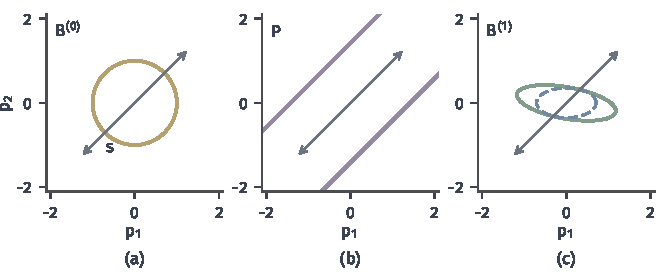
\includegraphics[width=112mm]{figures/05-optimization/02-smooth-optimization/matplotlib/qn-bfgs-strip/figure.pdf}
  \caption{贯穿例第一次BFGS更新的两步，曲线都是集合$\{\bm{p}:\bm{p}^\top\bm{M}\bm{p}=1\}$，箭头是$\bm{s}^{(0)}$所在的直线。(a)$\bm{M}=\bm{B}^{(0)}=\bm{I}$。(b)$\bm{M}=\bm{P}$，沿$\bm{s}$的曲率被清空，等值线变成平行的两条直线（紫）。(c)$\bm{M}=\bm{B}^{(1)}$（绿），加上测量项后重新合拢；蓝色虚线是真实Hessian的等值线。}
  \label{fig:qn-bfgs-strip}
\end{BookInlineFigure}

\paragraph{主要思想：对偶的DFP}
把同样的推导用在逆矩阵上。设$\bm{W}^{+}$是$\bm{W}$加上两个对称秩一项，代入割线条件~\eqref{eq:qn-secant-inverse}，取一项产生$\bm{s}$，另一项抵消$\bm{W}\bm{y}$，得到\term{DFP更新}（DFP update）：
\begin{equation}
 \bm{W}^{+}=\bm{W}-\frac{\bm{W}\bm{y}\bm{y}^\top\bm{W}}{\bm{y}^\top\bm{W}\bm{y}}+\rho\,\bm{s}\bm{s}^\top.
 \label{eq:qn-dfp-inverse}
\end{equation}
名称取自Davidon、Fletcher和Powell三人。对比式~\eqref{eq:qn-bfgs-direct}，两者互为对偶：在一个公式里交换$\bm{B}\leftrightarrow\bm{W}$、$\bm{s}\leftrightarrow\bm{y}$，就得到另一个。

实际计算只需要$\bm{W}$，方向~\eqref{eq:qn-direction}才不用解方程。DFP本来就是$\bm{W}$的公式，BFGS却要从$\bm{B}$翻译过来。下面的定理给出翻译的结果。

\begin{theorem}[BFGS的逆形式]
\label{thm:qn-bfgs-inverse}
设$\bm{B}\succ\bm{0}$，$\bm{W}=\bm{B}^{-1}$，$\bm{s}\neq\bm{0}$，$\langle\bm{s},\bm{y}\rangle>0$，并记$\bm{V}=\bm{I}-\rho\,\bm{y}\bm{s}^\top$。则式~\eqref{eq:qn-bfgs-direct}的$\bm{B}^{+}$可逆，其逆是
\begin{equation}
 \bm{W}^{+}=\bm{V}^\top\bm{W}\bm{V}+\rho\,\bm{s}\bm{s}^\top.
 \label{eq:qn-bfgs-inverse}
\end{equation}
\end{theorem}

\begin{proof}
只需验证$\bm{B}^{+}\bm{W}^{+}=\bm{I}$。先处理$\bm{B}^{+}\bm{V}^\top$。因为$\bm{V}^\top=\bm{I}-\rho\,\bm{s}\bm{y}^\top$，且$\bm{B}^{+}\bm{s}=\bm{y}$，所以
\[
 \bm{B}^{+}\bm{V}^\top=\bm{B}^{+}-\rho\,\bm{y}\bm{y}^\top=\bm{P}.
\]

再乘$\bm{W}$，由$\bm{B}\bm{W}=\bm{I}$，得到
\[
 \bm{P}\bm{W}=\bm{I}-\frac{\bm{B}\bm{s}\bm{s}^\top}{\bm{s}^\top\bm{B}\bm{s}}.
\]

接着由$\rho$的定义计算$\bm{s}^\top\bm{V}$：
\[
 \bm{s}^\top\bm{V}=\bm{s}^\top-\rho\langle\bm{s},\bm{y}\rangle\bm{s}^\top=\bm{0}^\top.
\]

所以右乘$\bm{V}$时第二项消失：
\[
 \bm{P}\bm{W}\bm{V}=\bm{V}.
\]

最后合并$\bm{W}^{+}$的两部分，并再用一次$\bm{B}^{+}\bm{s}=\bm{y}$：
\[
 \bm{B}^{+}\bm{W}^{+}=\bm{P}\bm{W}\bm{V}+\rho\,\bm{B}^{+}\bm{s}\bm{s}^\top=\bm{V}+\rho\,\bm{y}\bm{s}^\top=\bm{I}.
\]
方阵有右逆即可逆，定理得证。
\end{proof}

同样的公式也可以两次使用Sherman--Morrison公式得到，秩一修正求逆的公式可参考\BookChapterRef{chap:direct-linear-solvers}{卷二第12章“线性方程的直接求解”}。对偶地，DFP的直接形式是
\begin{equation}
 \bm{B}^{+}=\bm{V}\bm{B}\bm{V}^\top+\rho\,\bm{y}\bm{y}^\top.
 \label{eq:qn-dfp-direct}
\end{equation}

\paragraph{主要思想：新测量取代旧记忆}
逆形式~\eqref{eq:qn-bfgs-inverse}有一个清楚的解释。任取向量$\bm{z}$，令$a=\rho\langle\bm{s},\bm{z}\rangle$，由$\bm{V}$的定义，
\begin{equation}
 \bm{z}=a\,\bm{y}+\bm{V}\bm{z},\qquad\langle\bm{s},\bm{V}\bm{z}\rangle=0.
 \label{eq:qn-z-decomposition}
\end{equation}
也就是说，$\bm{z}$被拆成沿$\bm{y}$的部分和与$\bm{s}$正交的部分（这个拆分不是正交分解）。

把$\bm{W}^{+}$作用到$\bm{z}$上，得到
\[
 \bm{W}^{+}\bm{z}=a\,\bm{s}+\bm{V}^\top\bm{W}\bm{V}\bm{z}.
\]
沿$\bm{y}$的部分直接按测量结果换成$\bm{s}$，这正是割线条件；其余部分仍用旧矩阵$\bm{W}$处理，只是最后用$\bm{V}^\top$投影到$\bm{y}$的正交补上。图~\ref{fig:qn-bfgs-decomposition}画出了这个分解。

\begin{BookInlineFigure}
  \centering
  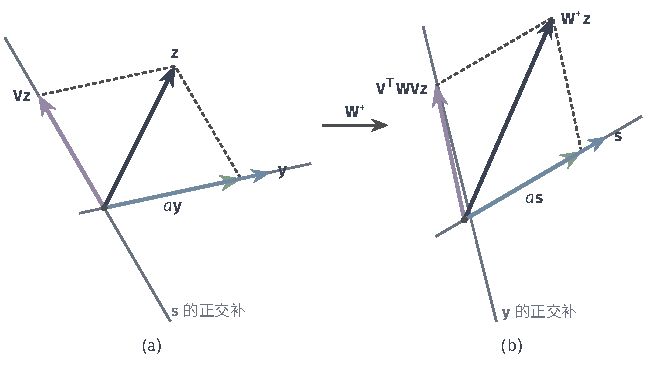
\includegraphics[width=108mm]{figures/05-optimization/02-smooth-optimization/tikz/qn-bfgs-decomposition/figure.pdf}
  \caption{BFGS逆更新对向量$\bm{z}$的作用，示意中旧矩阵取$\bm{W}=\bm{I}$。(a)$\bm{z}$沿$\bm{y}$与$\bm{s}$的正交补拆成两部分。(b)沿$\bm{y}$的部分$a\bm{y}$被换成$a\bm{s}$（绿），其余部分经旧矩阵后落在$\bm{y}$的正交补上（紫），两者相加得到$\bm{W}^{+}\bm{z}$。}
  \label{fig:qn-bfgs-decomposition}
\end{BookInlineFigure}

BFGS还有一个“改动最小”的刻画，它说明了在割线条件的整个解族中为什么选这一个。设$\bm{G}$是任意满足$\bm{G}\bm{s}=\bm{y}$的对称正定矩阵，例如$\bar{\bm{H}}$正定时的平均Hessian。在所有满足$\bm{W}=\bm{W}^\top$、$\bm{W}\bm{y}=\bm{s}$的矩阵中，BFGS的$\bm{W}^{+}$使加权距离$\lVert\bm{G}^{1/2}(\bm{W}-\bm{W}_{\mathrm{old}})\bm{G}^{1/2}\rVert_F$最小。

对偶地，DFP的$\bm{B}^{+}$在类似的约束下使$\lVert\bm{G}^{-1/2}(\bm{B}-\bm{B}_{\mathrm{old}})\bm{G}^{-1/2}\rVert_F$最小。证明需要把加权范数下的投影算出来，篇幅较长，读者可查阅\scite{math-nocedal2006numerical}。它的含义是：两种更新都尽量保留旧矩阵，只是一个在逆矩阵上度量改动，另一个在矩阵本身上度量改动。

\paragraph{曲率条件保证正定}
上一节说明曲率条件~\eqref{eq:qn-curvature-condition}是正定性的必要条件。现在证明，对BFGS和DFP它也是充分的。

\begin{theorem}[正定性的保持]
\label{thm:qn-positive-definite}
设$\bm{W}\succ\bm{0}$，$\bm{s}\neq\bm{0}$，$\bm{y}\neq\bm{0}$。则BFGS的$\bm{W}^{+}$与DFP的$\bm{W}^{+}$都正定，当且仅当$\langle\bm{s},\bm{y}\rangle>0$。
\end{theorem}

\begin{proof}
必要性：割线条件$\bm{W}^{+}\bm{y}=\bm{s}$与$\bm{y}$作内积，得到
\[
 \bm{y}^\top\bm{W}^{+}\bm{y}=\langle\bm{s},\bm{y}\rangle.
\]
若$\bm{W}^{+}\succ\bm{0}$，左边为正。

BFGS的充分性：对任意$\bm{z}\neq\bm{0}$，由式~\eqref{eq:qn-bfgs-inverse}，
\[
 \bm{z}^\top\bm{W}^{+}\bm{z}=(\bm{V}\bm{z})^\top\bm{W}(\bm{V}\bm{z})+\rho\langle\bm{s},\bm{z}\rangle^2.
\]
两项都非负。若第二项为零，则$\langle\bm{s},\bm{z}\rangle=0$，此时$\bm{V}\bm{z}=\bm{z}\neq\bm{0}$，第一项严格为正；所以和严格为正。

DFP的充分性：式~\eqref{eq:qn-dfp-direct}在结构上就是把式~\eqref{eq:qn-bfgs-inverse}中的$(\bm{W},\bm{s},\bm{y})$换成$(\bm{B},\bm{y},\bm{s})$，同样的论证给出$\bm{B}^{+}\succ\bm{0}$，因而$\bm{W}^{+}\succ\bm{0}$。
\end{proof}

\paragraph{Wolfe线搜索的作用}
剩下的问题是让曲率条件真的成立。第~\ref{sec:qn-secant}节留下的第二条Wolfe不等式正是为此准备的。记$\bm{s}=\alpha\bm{d}$，用第二条不等式，得到
\[
 \langle\bm{y},\bm{d}\rangle=\langle\bm{g}^{+},\bm{d}\rangle-\langle\bm{g},\bm{d}\rangle\geq(c_2-1)\langle\bm{g},\bm{d}\rangle.
\]
再乘以$\alpha>0$，由$c_2<1$和$\langle\bm{g},\bm{d}\rangle<0$，右端为正，于是
\begin{equation}
 \langle\bm{s},\bm{y}\rangle\geq\alpha(c_2-1)\langle\bm{g},\bm{d}\rangle>0.
 \label{eq:qn-wolfe-curvature}
\end{equation}
所以Wolfe线搜索对任意光滑目标都保证曲率条件，不需要目标是凸的。

只有充分下降条件是不够的。图~\ref{fig:qn-wolfe-curvature}取一维函数$\phi(\alpha)=f(\bm{x}+\alpha\bm{d})$，其导数为$\phi'(\alpha)=-1-1.5\alpha+\alpha^3$，它在起点附近向下弯。由$\bm{s}=\alpha\bm{d}$，曲率条件等价于$\phi'(\alpha)>\phi'(0)$。取$\alpha=0.5$，充分下降条件（$c_1=0.1$）成立，但
\[
 \phi'(0.5)=-1.625<-1=\phi'(0),
\]
曲率条件失败。取$c_2=0.5$时，第二条Wolfe不等式要求$\phi'(\alpha)\geq-0.5$，这把步长推到了$\alpha\geq1.37$，那里曲率的平均值已经为正。

\begin{BookInlineFigure}
  \centering
  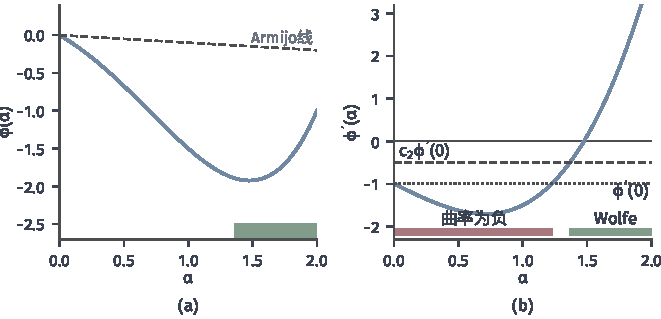
\includegraphics[width=112mm]{figures/05-optimization/02-smooth-optimization/matplotlib/qn-wolfe-curvature/figure.pdf}
  \caption{Wolfe条件怎样保证曲率条件，$\phi'(\alpha)=-1-1.5\alpha+\alpha^3$，$c_1=0.1$，$c_2=0.5$。(a)$\phi$（蓝）和充分下降的边界线（虚线），底部绿条是Wolfe条件的可接受步长。(b)$\phi'$（蓝）。红条上的步长满足$\phi'(\alpha)<\phi'(0)$，曲率条件失败；绿条上的步长满足$\phi'(\alpha)\geq c_2\phi'(0)$。}
  \label{fig:qn-wolfe-curvature}
\end{BookInlineFigure}

\paragraph{不用Wolfe时：跳过与阻尼}
有时线搜索只做回溯，或者步长由别的机制决定，曲率条件就可能不成立。这时有两种处理。

\textbf{跳过更新}：取小的正数$\varepsilon_{\mathrm{c}}$（如$10^{-8}$），当
\begin{equation}
 \langle\bm{s},\bm{y}\rangle\leq\varepsilon_{\mathrm{c}}\lVert\bm{s}\rVert_2\lVert\bm{y}\rVert_2
 \label{eq:qn-skip-rule}
\end{equation}
时令$\bm{W}^{+}=\bm{W}$。它保持正定，代价是这一次测量被扔掉。

\textbf{阻尼更新}：不扔掉测量，而是把$\bm{y}$与$\bm{B}\bm{s}$混合，使混合后的向量满足曲率要求。记曲率比
\[
 \tau=\frac{\langle\bm{s},\bm{y}\rangle}{\bm{s}^\top\bm{B}\bm{s}},
\]
再取
\begin{equation}
 \theta=\begin{cases}1,&\tau\geq0.2,\\\dfrac{0.8}{1-\tau},&\tau<0.2,\end{cases}\qquad
 \bm{r}=\theta\bm{y}+(1-\theta)\bm{B}\bm{s},
 \label{eq:qn-damping}
\end{equation}
再用$\bm{r}$代替$\bm{y}$代入式~\eqref{eq:qn-bfgs-direct}。

这样处理后$\tau<0.2$时的曲率比正好是$0.2$，因为
\[
 \frac{\langle\bm{s},\bm{r}\rangle}{\bm{s}^\top\bm{B}\bm{s}}=\theta\tau+1-\theta=1-\theta(1-\tau)=0.2.
\]
曲率比大于零，由定理~\ref{thm:qn-positive-definite}，$\bm{B}^{+}$正定。

用第~\ref{sec:qn-secant}节的不定例子算一次。取$\bm{B}=\bm{I}$，$\bm{s}=(1,2)^\top$，$\bm{y}=(2,-2)^\top$，则$\bm{s}^\top\bm{B}\bm{s}=5$，$\tau=-0.4$，于是
\[
 \theta=\frac{0.8}{1.4}=\frac47,\qquad
 \bm{r}=\frac47(2,-2)^\top+\frac37(1,2)^\top=\Bigl(\frac{11}{7},-\frac27\Bigr)^\top.
\]
验算：$\langle\bm{s},\bm{r}\rangle=11/7-4/7=1=0.2\times5$。图~\ref{fig:qn-damping}是$\theta$和修正前后曲率比的变化。

要注意阻尼放弃了什么：新矩阵满足$\bm{B}^{+}\bm{s}=\bm{r}$，而不再满足原来的割线条件。下表比较这三种机制。

\begin{BookInlineTable}
  \centering
  \begin{tabular}{lll}
    \toprule
    机制 & 曲率条件 & 代价\\
    \midrule
    Wolfe线搜索 & 由线搜索保证 & 可能多几次函数和梯度计算\\
    跳过更新 & 不成立时不更新 & 丢掉这次测量\\
    阻尼更新 & 由混合后的$\bm{r}$保证 & 放弃原来的割线条件\\
    \bottomrule
  \end{tabular}
  \caption{保持正定性的三种机制。}
  \label{tab:qn-curvature-mechanisms}
\end{BookInlineTable}

\begin{BookInlineFigure}
  \centering
  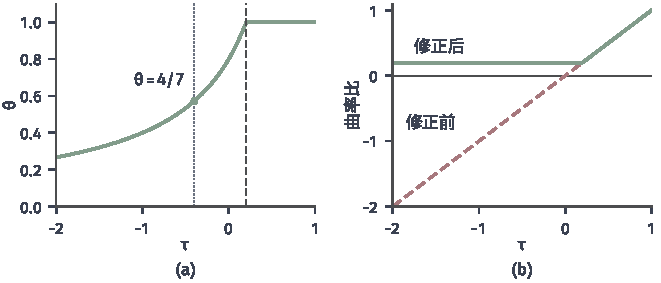
\includegraphics[width=112mm]{figures/05-optimization/02-smooth-optimization/matplotlib/qn-damping/figure.pdf}
  \caption{阻尼更新。(a)式~\eqref{eq:qn-damping}中的混合系数$\theta$随曲率比$\tau$的变化，虚线是阈值$\tau=0.2$，绿点是例中的$\tau=-0.4$，$\theta=4/7$。(b)修正前（红虚线）与修正后（绿）的曲率比，修正后不低于$0.2$。}
  \label{fig:qn-damping}
\end{BookInlineFigure}

\paragraph{计算过程}
下面用贯穿例~\eqref{eq:qn-running-example}完整走一遍BFGS，步长取精确线搜索，它在二次目标上满足Wolfe条件。

\needspace{6\baselineskip}
\paragraph{变量}
\begin{itemize}
 \item $\bm{x}^{(t)}\in\mathbb{R}^{n}$：当前迭代点；$\bm{g}^{(t)}\in\mathbb{R}^{n}$：当前梯度。
 \item $\bm{W}^{(t)}\in\mathbb{R}^{n\times n}$：对称正定的逆曲率近似。
 \item $\bm{d}^{(t)}$、$\alpha^{(t)}$：方向与步长。
 \item $\bm{s}^{(t)}$、$\bm{y}^{(t)}\in\mathbb{R}^{n}$、$\rho^{(t)}$：位移、梯度差与$1/\langle\bm{s}^{(t)},\bm{y}^{(t)}\rangle$。
\end{itemize}

\paragraph{初始化}
选起点$\bm{x}^{(0)}$和对称正定的$\bm{W}^{(0)}$，通常取单位矩阵的倍数，并计算$\bm{g}^{(0)}$。例中初始数据是
\[
 \bm{x}^{(0)}=(4,1)^\top,\qquad\bm{W}^{(0)}=\bm{I},\qquad\bm{g}^{(0)}=(8,8)^\top.
\]

\paragraph{每轮更新}
对$t=0,1,\ldots$依次执行下面的步骤，当$\lVert\bm{g}^{(t)}\rVert_2\leq\varepsilon$时停止。

\begin{enumerate}
\item 由式~\eqref{eq:qn-direction}计算方向$\bm{d}^{(t)}=-\bm{W}^{(t)}\bm{g}^{(t)}$。例中第一轮$\bm{d}^{(0)}=(-8,-8)^\top$。

\item 沿$\bm{d}^{(t)}$做满足式~\eqref{eq:qn-wolfe}的线搜索，优先试$\alpha=1$。例中用精确线搜索，第一轮的步长是
\[
 \alpha^{(0)}=\frac15.
\]

\item 更新迭代点并计算新梯度。例中第一轮得到
\[
 \bm{x}^{(1)}=(2.4,-0.6)^\top,\qquad\bm{g}^{(1)}=(4.8,-4.8)^\top.
\]

\item 由式~\eqref{eq:qn-s-y}计算$\bm{s}^{(t)}$、$\bm{y}^{(t)}$和$\rho^{(t)}$，并检查曲率条件。例中第一轮的$\bm{s}^{(0)}$、$\bm{y}^{(0)}$由式~\eqref{eq:qn-running-pair}给出，且
\[
 \langle\bm{s}^{(0)},\bm{y}^{(0)}\rangle=25.6,\qquad\rho^{(0)}=\frac{1}{25.6}.
\]

\item 用$\bm{s}^{(t)}$、$\bm{y}^{(t)}$、$\rho^{(t)}$构成定理~\ref{thm:qn-bfgs-inverse}中的$\bm{V}$，由式~\eqref{eq:qn-bfgs-inverse}更新$\bm{W}^{(t+1)}$。例中第一轮的两个中间量是
\[
 \bm{V}=\begin{bmatrix}0.8&-0.2\\-0.8&0.2\end{bmatrix},\qquad
 \rho^{(0)}\bm{s}^{(0)}\bigl(\bm{s}^{(0)}\bigr)^\top=\begin{bmatrix}0.1&0.1\\0.1&0.1\end{bmatrix}.
\]
由此得到
\[
 \bm{W}^{(1)}=\bm{V}^\top\bm{V}+\rho^{(0)}\bm{s}^{(0)}\bigl(\bm{s}^{(0)}\bigr)^\top
 =\begin{bmatrix}1.38&-0.22\\-0.22&0.18\end{bmatrix}.
\]
\end{enumerate}

$\bm{W}^{(1)}$的逆是
\[
 \bm{B}^{(1)}=\begin{bmatrix}0.9&1.1\\1.1&6.9\end{bmatrix},
\]
即族~\eqref{eq:qn-secant-family}中$a=0.9$的成员。验算割线条件，$\bm{W}^{(1)}\bm{y}^{(0)}$算出来确实是$(-1.6,-1.6)^\top$，也就是$\bm{s}^{(0)}$。

第二轮按同样的步骤进行。方向和精确步长是
\[
 \bm{d}^{(1)}=-\bm{W}^{(1)}\bm{g}^{(1)}=(-7.68,1.92)^\top,\qquad\alpha^{(1)}=\frac{46.08}{147.456}=\frac{5}{16}.
\]

于是迭代点到达
\[
 \bm{x}^{(2)}=\bm{x}^{(1)}+\alpha^{(1)}\bm{d}^{(1)}=(0,0)^\top,\qquad\bm{g}^{(2)}=\bm{0}.
\]
梯度为零，迭代结束。

为了看矩阵学到了什么，再做一次更新。这时有
\[
 \bm{s}^{(1)}=(-2.4,0.6)^\top,\qquad\bm{y}^{(1)}=(-4.8,4.8)^\top,\qquad\rho^{(1)}=\frac{1}{14.4}.
\]

由式~\eqref{eq:qn-bfgs-inverse}得到
\[
 \bm{W}^{(2)}=\begin{bmatrix}0.5&0\\0&0.125\end{bmatrix}=\bm{A}^{-1}.
\]
最终得到解$\bm{x}^{(2)}=\bm{0}$，而且两次测量之后逆曲率近似恰好等于真实Hessian的逆。图~\ref{fig:qn-bfgs-path}展示了路径和矩阵的变化。

\begin{BookInlineFigure}
  \centering
  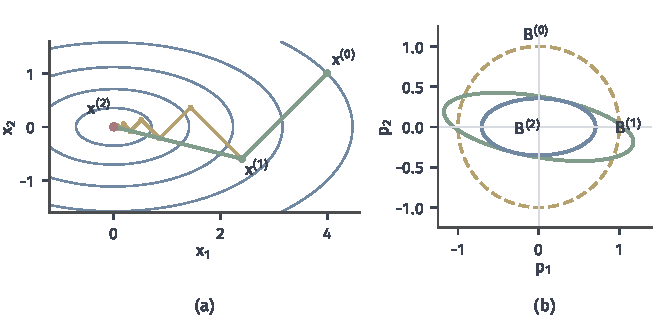
\includegraphics[width=112mm]{figures/05-optimization/02-smooth-optimization/matplotlib/qn-bfgs-path/figure.pdf}
  \caption{贯穿例上的BFGS。(a)蓝线是$f(\bm{x})=x_1^2+4x_2^2$的等高线，绿线是BFGS（$\bm{W}^{(0)}=\bm{I}$，精确线搜索）的两步，黄线是相同起点的最速下降。(b)集合$\{\bm{p}:\bm{p}^\top\bm{B}^{(t)}\bm{p}=1\}$，从圆（黄虚线）经过倾斜的椭圆（绿）变成真实Hessian的等值线（蓝）。}
  \label{fig:qn-bfgs-path}
\end{BookInlineFigure}

这不是巧合。在正定二次目标上使用精确线搜索时，BFGS产生的方向两两关于Hessian共轭，至多$n$步到达最优解，并且$\bm{W}^{(n)}=\bm{A}^{-1}$；第二次更新也没有破坏第一次的测量，例中可以验算$\bm{W}^{(2)}\bm{y}^{(0)}=\bm{s}^{(0)}$。证明用对步数的归纳法，篇幅较长，读者可查阅\scite{math-nocedal2006numerical}。这个结论依赖精确线搜索和二次目标，一般目标上不成立。

\paragraph{DFP与BFGS的对比}
用同一个例子算DFP。第一轮的$\bm{s}^{(0)}$、$\bm{y}^{(0)}$相同，由式~\eqref{eq:qn-dfp-inverse}得到
\[
 \bm{W}^{(1)}_{\mathrm{DFP}}=\frac{1}{170}\begin{bmatrix}177&-23\\-23&27\end{bmatrix}.
\]
它的逆是族~\eqref{eq:qn-secant-family}中$a=1.08$的成员。

矩阵不同，第二轮的方向却平行，$\bm{d}^{(1)}_{\mathrm{DFP}}$约为$(-5.647,1.412)^\top$，正好是BFGS方向的$0.735$倍。原因在于精确线搜索使$\langle\bm{g}^{(1)},\bm{s}^{(0)}\rangle=0$，再由割线条件和$\bm{d}^{(1)}=-\bm{W}^{(1)}\bm{g}^{(1)}$，得到
\[
 \langle\bm{y}^{(0)},\bm{d}^{(1)}\rangle=-\langle\bm{W}^{(1)}\bm{y}^{(0)},\bm{g}^{(1)}\rangle=-\langle\bm{s}^{(0)},\bm{g}^{(1)}\rangle=0.
\]
二维时这确定了方向。两种方法在这个例子上走过完全相同的点。

一旦线搜索不精确，差别就显现出来。图~\ref{fig:qn-dfp-bfgs-scaling}在一个$10$维强凸目标上比较两者，线搜索都满足强Wolfe条件。初始矩阵取$\bm{I}$时，两者都在约$20$步内收敛。

把初始矩阵缩小为$10^{-3}\bm{I}$，相当于矩阵$\bm{B}^{(0)}$的曲率估计过大，BFGS用$74$步恢复，DFP在$300$步后梯度大小仍约为$3.9$。这种从错误的曲率估计中恢复的能力称为自校正。第~\ref{sec:qn-convergence}节会用一个势函数解释BFGS的自校正，那个论证对DFP不适用。这就是实践中通常用BFGS而不用DFP的原因。

\begin{BookInlineFigure}
  \centering
  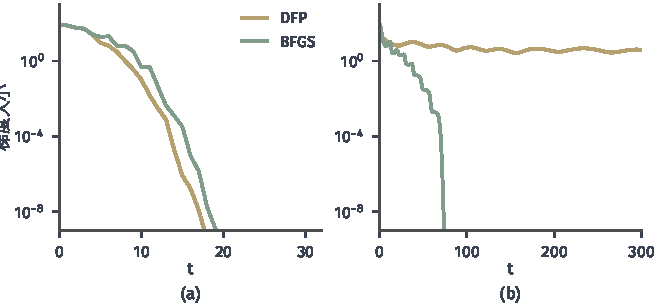
\includegraphics[width=112mm]{figures/05-optimization/02-smooth-optimization/matplotlib/qn-dfp-bfgs-scaling/figure.pdf}
  \caption{BFGS（绿）与DFP（黄）的梯度大小随迭代的变化。目标是$10$维强凸函数$\sum_i(\tfrac12c_iz_i^2+\ln\cosh z_i)$，其中$\bm{z}=\bm{Q}\bm{x}$，$\bm{Q}$是固定的正交矩阵，$c_i$在$[0.1,100]$上对数等距；线搜索为强Wolfe条件，$c_1=10^{-4}$，$c_2=0.9$。(a)$\bm{W}^{(0)}=\bm{I}$。(b)$\bm{W}^{(0)}=10^{-3}\bm{I}$，注意横轴范围不同。}
  \label{fig:qn-dfp-bfgs-scaling}
\end{BookInlineFigure}

\section{SR1}
\label{sec:qn-sr1}

BFGS为了保持正定，把负曲率的测量拒之门外。可是目标在某些方向确实向下弯时，这恰恰是有用的信息。这就需要回答：只用一个秩一项能否满足割线条件，这样得到的矩阵有什么长处，又有什么风险？

\paragraph{主要思想：只有一种秩一修正}
设$\bm{B}^{+}=\bm{B}+\sigma\bm{v}\bm{v}^\top$，其中$\sigma=\pm1$。记割线残差$\bm{r}=\bm{y}-\bm{B}\bm{s}$，把割线条件写成
\[
 \sigma\langle\bm{v},\bm{s}\rangle\bm{v}=\bm{r}.
\]
左边是$\bm{v}$的数乘，所以$\bm{v}$必须平行于$\bm{r}$。把$\bm{v}$取成$\bm{r}$的倍数后，$\sigma$和倍数只有一种可能，由此得到\term{对称秩一更新}（symmetric rank-one update，SR1）：
\begin{equation}
 \bm{B}^{+}=\bm{B}+\frac{\bm{r}\bm{r}^\top}{\langle\bm{r},\bm{s}\rangle},\qquad\bm{r}=\bm{y}-\bm{B}\bm{s}.
 \label{eq:qn-sr1-direct}
\end{equation}

与第~\ref{sec:qn-dfp-bfgs}节不同，这里的更新由割线条件和“秩一”完全确定，没有选择余地。验算割线条件：$\bm{B}^{+}\bm{s}=\bm{B}\bm{s}+\bm{r}=\bm{y}$。

把同样的推导用在逆矩阵上，并记$\bm{w}=\bm{s}-\bm{W}\bm{y}$，得到
\begin{equation}
 \bm{W}^{+}=\bm{W}+\frac{\bm{w}\bm{w}^\top}{\langle\bm{w},\bm{y}\rangle}.
 \label{eq:qn-sr1-inverse}
\end{equation}
只要$\bm{B}$、$\bm{B}^{+}$都可逆，式~\eqref{eq:qn-sr1-inverse}的$\bm{W}^{+}$就是式~\eqref{eq:qn-sr1-direct}的$\bm{B}^{+}$的逆，这可以用Sherman--Morrison公式验证。SR1自己是自己的对偶，所以不像BFGS和DFP那样分成两种方法。

\paragraph{计算过程}
SR1不需要线搜索来保持什么性质，下面就用单位步长演示它。仍用贯穿例，这一次不做线搜索，每步直接走完整的$-\bm{W}^{(t)}\bm{g}^{(t)}$。

\needspace{6\baselineskip}
\paragraph{变量}
\begin{itemize}
 \item $\bm{x}^{(t)}$、$\bm{g}^{(t)}\in\mathbb{R}^{n}$：当前点与梯度。
 \item $\bm{W}^{(t)}\in\mathbb{R}^{n\times n}$：对称的逆曲率近似，不要求正定。
 \item $\bm{s}^{(t)}$、$\bm{y}^{(t)}$：位移与梯度差；$\bm{w}^{(t)}$：式~\eqref{eq:qn-sr1-inverse}中逆形式的割线残差。
 \item $c_{\mathrm{r}}>0$：判断分母是否过小的阈值。
\end{itemize}

\paragraph{初始化}
选起点和对称的$\bm{W}^{(0)}$。例中初始数据是
\[
 \bm{x}^{(0)}=(4,1)^\top,\qquad\bm{W}^{(0)}=\bm{I},\qquad\bm{g}^{(0)}=(8,8)^\top.
\]

\paragraph{每轮更新}
对$t=0,1,\ldots$依次执行下面的步骤，当$\lVert\bm{g}^{(t)}\rVert_2\leq\varepsilon$时停止。

\begin{enumerate}
\item 计算$\bm{s}^{(t)}=-\bm{W}^{(t)}\bm{g}^{(t)}$，令$\bm{x}^{(t+1)}=\bm{x}^{(t)}+\bm{s}^{(t)}$，并读取$\bm{g}^{(t+1)}$。例中第一轮得到
\[
 \bm{s}^{(0)}=(-8,-8)^\top,\qquad\bm{x}^{(1)}=(-4,-7)^\top,\qquad\bm{g}^{(1)}=(-8,-56)^\top.
\]
目标值从$20$升到了$212$，这一步在目标上是失败的，但测量仍然有用。

\item 计算$\bm{y}^{(t)}=\bm{g}^{(t+1)}-\bm{g}^{(t)}$和$\bm{w}^{(t)}$。例中第一轮得到
\[
 \bm{y}^{(0)}=(-16,-64)^\top,\qquad\bm{w}^{(0)}=(8,56)^\top,\qquad\langle\bm{w}^{(0)},\bm{y}^{(0)}\rangle=-3712.
\]

\item 若$\langle\bm{w}^{(t)},\bm{y}^{(t)}\rangle$的绝对值不小于$c_{\mathrm{r}}\lVert\bm{w}^{(t)}\rVert_2\lVert\bm{y}^{(t)}\rVert_2$，由式~\eqref{eq:qn-sr1-inverse}更新$\bm{W}^{(t+1)}$；否则令$\bm{W}^{(t+1)}=\bm{W}^{(t)}$。例中第一轮分母足够大，更新后得到
\[
 \bm{W}^{(1)}=\frac{1}{58}\begin{bmatrix}57&-7\\-7&9\end{bmatrix}.
\]
\end{enumerate}

第二轮的位移与新点是
\[
 \bm{s}^{(1)}=\frac{1}{29}(32,224)^\top,\qquad\bm{x}^{(2)}=\frac{1}{29}(-84,21)^\top\approx(-2.897,0.724)^\top.
\]

梯度差和逆形式残差是
\[
 \bm{y}^{(1)}=\frac{1}{29}(64,1792)^\top,\qquad\bm{w}^{(1)}=\frac{1344}{841}(4,-1)^\top.
\]

分母约为$-84.64$，更新量是$-\tfrac{7}{232}$乘以$\begin{bmatrix}16&-4\\-4&1\end{bmatrix}$，于是
\[
 \bm{W}^{(2)}=\begin{bmatrix}0.5&0\\0&0.125\end{bmatrix}=\bm{A}^{-1}.
\]

第三轮的方向已经是Newton方向，一步到达解：
\[
 \bm{s}^{(2)}=\frac{1}{29}(84,-21)^\top,\qquad\bm{x}^{(3)}=\bm{0},\qquad\bm{g}^{(3)}=\bm{0}.
\]
迭代结束，最终得到解$\bm{x}^{(3)}=\bm{0}$，用了$n+1=3$步。图~\ref{fig:qn-sr1-path}是这条路径。

\begin{BookInlineFigure}
  \centering
  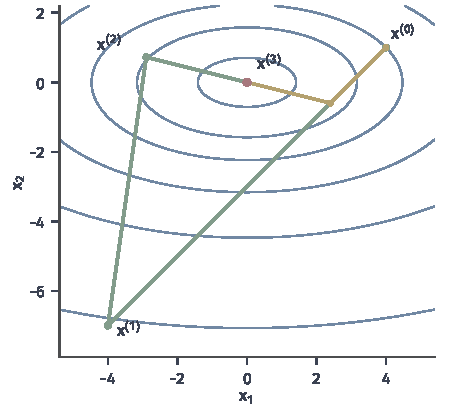
\includegraphics[width=78mm]{figures/05-optimization/02-smooth-optimization/matplotlib/qn-sr1-path/figure.pdf}
  \caption{贯穿例上的SR1路径（绿）：$\bm{W}^{(0)}=\bm{I}$，每步取单位步长。第一步远远越过谷底，目标值从$20$升到$212$，但两次测量足以确定$\bm{A}$，第三步准确落在最优解（红）。黄线是精确线搜索的BFGS路径，用作对照。}
  \label{fig:qn-sr1-path}
\end{BookInlineFigure}

\paragraph{有限步终止}
这个现象对二次目标普遍成立，而且完全不依赖步长的选取。下面的定理把BFGS那里“两次测量都不丢失”的现象，以更强的形式写了下来。

\begin{theorem}[SR1的遗传性质]
\label{thm:qn-sr1-hereditary}
设$f$是二次函数，Hessian为对称矩阵$\bm{A}$，于是$\bm{y}^{(j)}=\bm{A}\bm{s}^{(j)}$。设$\bm{B}^{(j+1)}$由SR1按式~\eqref{eq:qn-sr1-direct}逐次得到，所有分母非零。则对每个$k$，
\begin{equation}
 \bm{B}^{(k)}\bm{s}^{(j)}=\bm{y}^{(j)},\qquad j=0,1,\ldots,k-1.
 \label{eq:qn-sr1-hereditary}
\end{equation}
特别地，若$\bm{s}^{(0)},\ldots,\bm{s}^{(n-1)}$线性无关，则$\bm{B}^{(n)}=\bm{A}$。
\end{theorem}

\begin{proof}
对$k$归纳。$k=1$时就是割线条件。设式~\eqref{eq:qn-sr1-hereditary}对$k$成立，并记$\bm{r}=\bm{y}^{(k)}-\bm{B}^{(k)}\bm{s}^{(k)}$。

对$j<k$，由归纳假设、对称性和$\bm{y}^{(j)}=\bm{A}\bm{s}^{(j)}$，得到
\[
 \begin{aligned}
 \langle\bm{r},\bm{s}^{(j)}\rangle
 &=\langle\bm{y}^{(k)},\bm{s}^{(j)}\rangle-\langle\bm{s}^{(k)},\bm{B}^{(k)}\bm{s}^{(j)}\rangle\\
 &=\langle\bm{A}\bm{s}^{(k)},\bm{s}^{(j)}\rangle-\langle\bm{s}^{(k)},\bm{A}\bm{s}^{(j)}\rangle=0.
 \end{aligned}
\]

所以秩一修正项作用在旧位移上为零：
\[
 \bm{B}^{(k+1)}\bm{s}^{(j)}=\bm{B}^{(k)}\bm{s}^{(j)}+\bm{r}\,\frac{\langle\bm{r},\bm{s}^{(j)}\rangle}{\langle\bm{r},\bm{s}^{(k)}\rangle}=\bm{y}^{(j)}.
\]
$j=k$时是割线条件本身，归纳完成。

$\bm{s}^{(j)}$线性无关时，把它们排成可逆矩阵$\bm{S}$，式~\eqref{eq:qn-sr1-hereditary}说明$\bm{B}^{(n)}\bm{S}=\bm{A}\bm{S}$，右乘$\bm{S}^{-1}$即得。
\end{proof}

所以$\bm{A}$可逆、$\bm{B}^{(n)}$之前的各步线性无关时，单位步长的SR1至多$n+1$步到达驻点。定理没有要求$\bm{A}$正定，也没有要求线搜索，这是SR1与BFGS的重要区别。

\paragraph{分母可能为零}
SR1的麻烦全在分母$\langle\bm{r},\bm{s}\rangle$上。若$\bm{r}\neq\bm{0}$而$\langle\bm{r},\bm{s}\rangle=0$，则根本不存在满足割线条件的对称秩一修正。原因是由$\sigma\langle\bm{v},\bm{s}\rangle\bm{v}=\bm{r}$与$\bm{s}$作内积，得到
\[
 \sigma\langle\bm{v},\bm{s}\rangle^2=\langle\bm{r},\bm{s}\rangle=0.
\]
于是$\langle\bm{v},\bm{s}\rangle=0$，等式左边就是零向量，与$\bm{r}\neq\bm{0}$矛盾。

这种情况确实会出现。取$\bm{A}=\operatorname{diag}(2,8)$，$\bm{B}=\operatorname{diag}(3,7)$，$\bm{s}=(1,1)^\top$，则
\[
 \bm{y}=(2,8)^\top,\qquad\bm{r}=(-1,1)^\top,\qquad\langle\bm{r},\bm{s}\rangle=0.
\]

分母接近零同样有害。把$\bm{s}$换成$(1,1+\epsilon)^\top$，分母是$2\epsilon+\epsilon^2$，而$\lVert\bm{r}\rVert_2$约为$\sqrt2$，修正量的Frobenius范数约为$1/\epsilon$。图~\ref{fig:qn-sr1-denominator}展示了这种放大：$\epsilon=10^{-4}$时修正量约为$10^{4}$，矩阵几乎被这一次修正淹没。

\begin{BookInlineFigure}
  \centering
  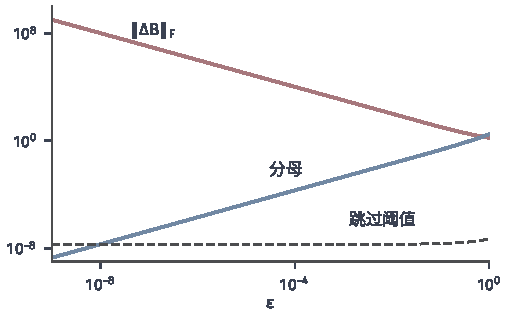
\includegraphics[width=86mm]{figures/05-optimization/02-smooth-optimization/matplotlib/qn-sr1-denominator/figure.pdf}
  \caption{SR1的分母接近零时的放大效应：$\bm{A}=\operatorname{diag}(2,8)$，$\bm{B}=\operatorname{diag}(3,7)$，$\bm{s}=(1,1+\epsilon)^\top$。蓝线是分母$\lvert\langle\bm{r},\bm{s}\rangle\rvert$，红线是修正量$\lVert\Delta\bm{B}\rVert_F$；虚线是取$c_{\mathrm{r}}=10^{-8}$时的跳过阈值$c_{\mathrm{r}}\lVert\bm{r}\rVert_2\lVert\bm{s}\rVert_2$，分母低于它就不更新。}
  \label{fig:qn-sr1-denominator}
\end{BookInlineFigure}

所以SR1配有跳过规则，这就是计算过程第三步的判断，直接形式下写成
\begin{equation}
 \lvert\langle\bm{r},\bm{s}\rangle\rvert\geq c_{\mathrm{r}}\lVert\bm{r}\rVert_2\lVert\bm{s}\rVert_2,
 \label{eq:qn-sr1-safeguard}
\end{equation}
通常取$c_{\mathrm{r}}=10^{-8}$。不满足时保持$\bm{B}^{+}=\bm{B}$。

式~\eqref{eq:qn-sr1-safeguard}中的角度形式比绝对阈值合理：它问的是$\bm{r}$与$\bm{s}$是否几乎垂直，与两个向量的长度无关。跳过很少发生，因为分母近零需要$\bm{r}$恰好几乎垂直于$\bm{s}$。

\paragraph{SR1通常不保持正定}
BFGS的更新中，分母$\langle\bm{s},\bm{y}\rangle$与修正项的符号都受控制。SR1的分母可正可负，修正项的符号跟着变，所以正定矩阵可能变成不定矩阵，即使目标强凸。

取贯穿例的目标，$\bm{x}^{(0)}=(-4,-0.5)^\top$，$\bm{B}^{(0)}=4\bm{I}$，单位步长。这时
\[
 \bm{g}^{(0)}=(-8,-4)^\top,\qquad\bm{s}^{(0)}=(2,1)^\top,\qquad\bm{y}^{(0)}=(4,8)^\top.
\]

$\bm{B}^{(0)}\bm{s}^{(0)}=(8,4)^\top$，所以残差和分母是
\[
 \bm{r}=(-4,4)^\top,\qquad\langle\bm{r},\bm{s}^{(0)}\rangle=-4.
\]
代入式~\eqref{eq:qn-sr1-direct}，得到
\[
 \bm{B}^{(1)}=\begin{bmatrix}0&4\\4&0\end{bmatrix}.
\]
它的特征值是$\pm4$，不定。验算割线条件：$\bm{B}^{(1)}\bm{s}^{(0)}=(4,8)^\top=\bm{y}^{(0)}$。

新点是$\bm{x}^{(1)}=(-2,0.5)^\top$，梯度$\bm{g}^{(1)}=(-4,4)^\top$。若仍然用公式~\eqref{eq:qn-direction}算方向，得到
\[
 \bm{d}=-\bigl(\bm{B}^{(1)}\bigr)^{-1}\bm{g}^{(1)}=(-1,1)^\top,\qquad\langle\bm{g}^{(1)},\bm{d}\rangle=8>0.
\]

这是一个上升方向。$\bm{d}$是模型的驻点，但模型不定，驻点是鞍点而不是极小点。沿它走一步，目标从$5$升到$18$。第~\ref{sec:qn-secant}节的下降论证依赖$\bm{W}$正定，这里前提已经不成立，所以不能把BFGS方向的下降分析搬过来。

\paragraph{不定模型与信赖域}
不定的$\bm{B}$并非无用，用错的只是“跑到模型驻点”这个做法。模型$m(\bm{p})$在$\bm{p}$的某些方向向下弯，这时它没有极小点，但在一个有界的范围内它有。第~\ref{chap:trust-region}章的信赖域方法正是如此：只在以当前点为中心、半径为$\Delta$的球内最小化模型，并用实际下降检验这个候选步。

继续上面的例子，取$\Delta=1$。$\bm{B}^{(1)}$的负特征值$-4$对应单位特征向量$\bm{v}=(1,-1)^\top/\sqrt2$，而$\bm{g}^{(1)}=-4\sqrt2\,\bm{v}$恰好全部落在这个方向上。沿$\bm{p}=\beta\bm{v}$，模型的变化量是
\[
 m(\beta\bm{v})-m(\bm{0})=-4\sqrt2\,\beta-2\beta^2.
\]

在$\lvert\beta\rvert\leq1$上它在$\beta=1$处最小，所以候选步是
\[
 \bm{p}_{\Delta}=\frac{1}{\sqrt2}(1,-1)^\top.
\]
它是下降方向，因为与梯度的内积是$-4\sqrt2<0$。沿它走一步，目标从$5$降到约$1.843$。图~\ref{fig:qn-sr1-saddle}比较了两个候选步。

\begin{BookInlineFigure}
  \centering
  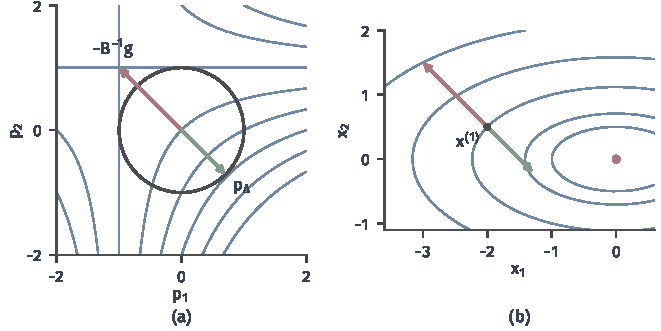
\includegraphics[width=112mm]{figures/05-optimization/02-smooth-optimization/matplotlib/qn-sr1-saddle/figure.pdf}
  \caption{不定模型下的两个候选步，$\bm{B}=\begin{bmatrix}0&4\\4&0\end{bmatrix}$，$\bm{g}=(-4,4)^\top$，圆的半径为$1$。(a)蓝线是模型$m(\bm{p})$的等值线，呈鞍形。红箭头是模型的驻点$-\bm{B}^{-1}\bm{g}$，绿箭头是圆内模型的极小点。(b)同样的两步放到真实目标$x_1^2+4x_2^2$的等高线上，红步使目标上升，绿步使目标下降。}
  \label{fig:qn-sr1-saddle}
\end{BookInlineFigure}

这也解释了SR1和BFGS的分工。BFGS的矩阵总是正定的，方向一定下降，配线搜索很自然；但它看不到负曲率，也只有测量满足曲率条件才能更新。SR1能记录负曲率，在二次目标上对步长没有要求，但需要有界的模型来消化不定性。

\begin{BookInlineTable}
  \centering
  \begin{tabular}{lll}
    \toprule
    比较项 & BFGS & SR1\\
    \midrule
    修正的秩 & 二 & 一\\
    更新的前提 & 曲率条件 & 分母不过小\\
    正定性 & 保持 & 通常不保持\\
    负曲率信息 & 不能表示 & 可以表示\\
    配套的全局化手段 & Wolfe线搜索 & 信赖域\\
    \bottomrule
  \end{tabular}
  \caption{BFGS与SR1的对比。}
  \label{tab:qn-bfgs-sr1}
\end{BookInlineTable}

\section{L-BFGS}
\label{sec:qn-lbfgs}

BFGS不必解方程，但仍要保存一个$n\times n$的稠密矩阵。$n=10^6$时这需要约$10^{12}$个元素的存储，通常根本放不下。不保存矩阵，能否仍然算出$\bm{W}^{(t)}\bm{g}^{(t)}$？

\paragraph{主要思想：只保留最近的测量}
BFGS的$\bm{W}^{(t)}$完全由$\bm{W}^{(0)}$和所有的$(\bm{s}^{(j)},\bm{y}^{(j)})$决定。旧测量在非二次目标上已经过时，于是\term{有限记忆BFGS}（limited-memory BFGS，L-BFGS）只保留最近$r$对，$r$称为记忆长度，常取$3$到$30$。

存储从约$n^2/2$个数降到$2rn$个数。每一轮都重新从一个简单的初始矩阵$\gamma^{(t)}\bm{I}$出发，把这$r$对依次用式~\eqref{eq:qn-bfgs-inverse}更新一遍，得到的矩阵就是这一轮的$\bm{W}^{(t)}$。

记下面$r$次更新的中间矩阵为$\bm{W}_{[j]}$，下标$j$从$t-r$走到$t$。起点和递推是
\begin{equation}
 \bm{W}_{[t-r]}=\gamma^{(t)}\bm{I},\qquad
 \bm{W}_{[j+1]}=\bigl(\bm{V}^{(j)}\bigr)^\top\bm{W}_{[j]}\bm{V}^{(j)}+\rho^{(j)}\bm{s}^{(j)}\bigl(\bm{s}^{(j)}\bigr)^\top,
 \label{eq:qn-lbfgs-recursion}
\end{equation}
其中$\bm{V}^{(j)}$由第$j$对向量按定理~\ref{thm:qn-bfgs-inverse}的方式构成，最后$\bm{W}^{(t)}=\bm{W}_{[t]}$。显式写出这些矩阵要$O(n^2)$的存储，我们其实只需要它乘一个向量的结果。

\paragraph{主要思想：两层递推}
令$\bm{q}_{[t]}=\bm{g}^{(t)}$，想算$\bm{W}_{[t]}\bm{q}_{[t]}$。把递推~\eqref{eq:qn-lbfgs-recursion}作用在向量$\bm{q}_{[j+1]}$上，先算出向右侧的两个量：
\[
 \xi^{(j)}=\rho^{(j)}\langle\bm{s}^{(j)},\bm{q}_{[j+1]}\rangle,\qquad
 \bm{q}_{[j]}=\bm{V}^{(j)}\bm{q}_{[j+1]}=\bm{q}_{[j+1]}-\xi^{(j)}\bm{y}^{(j)}.
\]

于是一次更新对向量的作用可以写成
\[
 \bm{W}_{[j+1]}\bm{q}_{[j+1]}=\bigl(\bm{V}^{(j)}\bigr)^\top\bm{W}_{[j]}\bm{q}_{[j]}+\xi^{(j)}\bm{s}^{(j)}.
\]
右端的$\bm{W}_{[j]}\bm{q}_{[j]}$是同样形式、但下标小一的问题。所以计算分两层：第一层让$j$从$t-1$递减到$t-r$，把$\bm{q}$一路算下去，记下所有$\xi^{(j)}$。

第一层走到底时，最内层的矩阵是$\gamma^{(t)}\bm{I}$，令$\bm{z}_{[t-r]}=\gamma^{(t)}\bm{q}_{[t-r]}$。记$\bm{z}_{[j]}=\bm{W}_{[j]}\bm{q}_{[j]}$，把$\bm{V}^{(j)}$的转置展开，得到第二层的递推：
\begin{equation}
 \eta^{(j)}=\rho^{(j)}\langle\bm{y}^{(j)},\bm{z}_{[j]}\rangle,\qquad
 \bm{z}_{[j+1]}=\bm{z}_{[j]}+\bigl(\xi^{(j)}-\eta^{(j)}\bigr)\bm{s}^{(j)}.
 \label{eq:qn-lbfgs-second-loop}
\end{equation}
第二层让$j$从$t-r$递增到$t-1$，最后的$\bm{z}_{[t]}$就是$\bm{W}^{(t)}\bm{g}^{(t)}$。这就是\term{双循环递推}（two-loop recursion），图~\ref{fig:qn-lbfgs-two-loop}是它的结构。

\begin{BookInlineFigure}
  \centering
  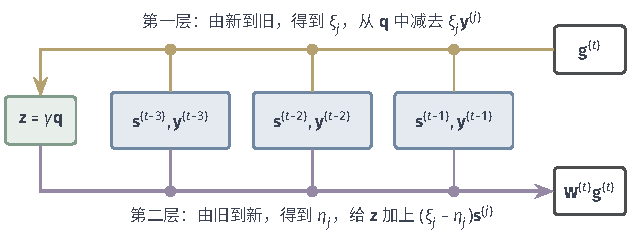
\includegraphics[width=106mm]{figures/05-optimization/02-smooth-optimization/tikz/qn-lbfgs-two-loop/figure.pdf}
  \caption{L-BFGS的双循环递推，$r=3$。蓝框是保存的三对向量。第一层（黄）从梯度出发，由最新一对走到最旧一对；中间乘初始矩阵$\gamma\bm{I}$（绿框）；第二层（紫）由最旧一对走回最新一对，输出$\bm{W}^{(t)}\bm{g}^{(t)}$。全程只有向量内积和向量加法。}
  \label{fig:qn-lbfgs-two-loop}
\end{BookInlineFigure}

每一层对每对向量做一次内积和一次向量加法，再加上中间的缩放，每个方向的运算量约为$(4r+1)n$次乘法。矩阵本身从未出现。

\paragraph{主要思想：初始缩放}
最内层的矩阵决定了双循环不了解的那些方向上的尺度。L-BFGS一般取
\begin{equation}
 \gamma^{(t)}=\frac{\langle\bm{s}^{(t-1)},\bm{y}^{(t-1)}\rangle}{\langle\bm{y}^{(t-1)},\bm{y}^{(t-1)}\rangle}.
 \label{eq:qn-lbfgs-gamma}
\end{equation}

它的含义可以由式~\eqref{eq:qn-average-hessian}看出。设平均Hessian正定，并把$(\bar{\bm{H}}^{(t-1)})^{1/2}\bm{s}^{(t-1)}$记作$\bm{z}$，则
\[
 \frac{1}{\gamma^{(t)}}=\frac{\bm{z}^\top\bar{\bm{H}}^{(t-1)}\bm{z}}{\bm{z}^\top\bm{z}}.
\]
所以$1/\gamma^{(t)}$是平均Hessian的一个Rayleigh商，落在其最小与最大特征值之间，是目标曲率的一个合理的标量估计。

\paragraph{主要思想：曲率检查}
与完整BFGS一样，存入的$(\bm{s}^{(j)},\bm{y}^{(j)})$必须满足$\langle\bm{s}^{(j)},\bm{y}^{(j)}\rangle>0$，否则式~\eqref{eq:qn-lbfgs-recursion}不再保证正定，算出的方向可能不下降。Wolfe线搜索使这一点自动成立。只用回溯时，要加上跳过规则：满足式~\eqref{eq:qn-skip-rule}的这一对不存入，窗口保持原样。

\paragraph{计算过程}
下面用贯穿例演示$r=2$的L-BFGS。为了不让第一层的系数因为正交性而消失，第一步取$\alpha^{(0)}=1/8$而不是精确步长，以后都用单位步长；这些步长都满足$c_1=10^{-4}$、$c_2=0.9$的Wolfe条件。

\needspace{6\baselineskip}
\paragraph{变量}
\begin{itemize}
 \item $\bm{x}^{(t)}$、$\bm{g}^{(t)}\in\mathbb{R}^{n}$：当前点与梯度。
 \item 窗口：最多$r$组$(\bm{s}^{(j)},\bm{y}^{(j)},\rho^{(j)})$，$\bm{s}^{(j)},\bm{y}^{(j)}\in\mathbb{R}^{n}$，$\rho^{(j)}$是标量，从旧到新排列。
 \item 第一层的向量$\bm{q}\in\mathbb{R}^{n}$和系数$\xi^{(j)}$；第二层的向量$\bm{z}\in\mathbb{R}^{n}$和系数$\eta^{(j)}$。
 \item $\gamma^{(t)}>0$：初始矩阵的缩放。
\end{itemize}

\paragraph{初始化}
选起点，窗口置空。窗口为空时取$\gamma^{(0)}=1$，方向就是负梯度。例中第一轮的数据是
\[
 \bm{x}^{(0)}=(4,1)^\top,\qquad\bm{g}^{(0)}=(8,8)^\top,\qquad\bm{d}^{(0)}=(-8,-8)^\top.
\]
取$\alpha^{(0)}=1/8$，走完后有
\[
 \bm{x}^{(1)}=(3,0)^\top,\qquad\bm{g}^{(1)}=(6,0)^\top.
\]
第一对测量及其$\rho$是
\[
 \bm{s}^{(0)}=(-1,-1)^\top,\qquad\bm{y}^{(0)}=(-2,-8)^\top,\qquad\rho^{(0)}=0.1.
\]

\paragraph{每轮更新}
对$t=1,2,\ldots$依次执行下面的步骤，当$\lVert\bm{g}^{(t)}\rVert_2\leq\varepsilon$时停止。

\begin{enumerate}
\item 第一层，令$\bm{q}=\bm{g}^{(t)}$，对窗口中的$j$由新到旧，依次计算
\[
 \xi^{(j)}=\rho^{(j)}\langle\bm{s}^{(j)},\bm{q}\rangle,\qquad\bm{q}\leftarrow\bm{q}-\xi^{(j)}\bm{y}^{(j)}.
\]
例中$t=1$时窗口只有一对，结果是
\[
 \xi^{(0)}=-0.6,\qquad\bm{q}=(4.8,-4.8)^\top.
\]

\item 由式~\eqref{eq:qn-lbfgs-gamma}计算$\gamma^{(t)}$，并令$\bm{z}=\gamma^{(t)}\bm{q}$。例中$t=1$时$\langle\bm{y}^{(0)},\bm{y}^{(0)}\rangle=68$，于是
\[
 \gamma^{(1)}=\frac{10}{68}=\frac{5}{34},\qquad\bm{z}\approx(0.7059,-0.7059)^\top.
\]

\item 第二层，对窗口中的$j$由旧到新，按式~\eqref{eq:qn-lbfgs-second-loop}更新$\bm{z}$。例中$t=1$时得到
\[
 \eta^{(0)}\approx0.4235,\qquad\bm{z}\approx(1.7294,0.3176)^\top.
\]

\item 令$\bm{d}^{(t)}=-\bm{z}$，线搜索后得到新点和新梯度。例中$t=1$时取$\alpha^{(1)}=1$，结果是
\[
 \bm{d}^{(1)}\approx(-1.7294,-0.3176)^\top,\qquad\bm{x}^{(2)}\approx(1.2706,-0.3176)^\top.
\]

\item 计算$\bm{s}^{(t)}$、$\bm{y}^{(t)}$和$\rho^{(t)}$，曲率检查通过后存入窗口；若窗口超过$r$对，丢弃最旧的一对。例中$t=1$时
\[
 \bm{y}^{(1)}\approx(-3.4588,-2.5412)^\top,\qquad\rho^{(1)}\approx0.14730.
\]
窗口现在有两对，还没有超过$r=2$。
\end{enumerate}

$t=2$时窗口有两对，能看到完整的双循环。此时的梯度是
\[
 \bm{g}^{(2)}\approx(2.5412,-2.5412)^\top.
\]
第一层由新到旧的两次计算是
\[
 \begin{aligned}
 j=1:&\quad\xi^{(1)}\approx-0.5284,\quad\bm{q}\approx(0.7134,-3.8840)^\top,\\
 j=0:&\quad\xi^{(0)}\approx0.3171,\quad\bm{q}\approx(1.3475,-1.3475)^\top.
 \end{aligned}
\]

中间的缩放使用最新一对，结果是
\[
 \gamma^{(2)}\approx0.36854,\qquad\bm{z}\approx(0.4966,-0.4966)^\top.
\]

第二层由旧到新的两次计算是
\[
 \begin{aligned}
 j=0:&\quad\eta^{(0)}\approx0.2980,\quad\bm{z}\approx(0.4775,-0.5157)^\top,\\
 j=1:&\quad\eta^{(1)}\approx-0.0503,\quad\bm{z}\approx(1.3045,-0.3638)^\top.
 \end{aligned}
\]

取单位步长，新的点是
\[
 \bm{d}^{(2)}\approx(-1.3045,0.3638)^\top,\qquad\bm{x}^{(3)}\approx(-0.0339,0.0462)^\top.
\]
$t=3$时窗口超过$r=2$，$\bm{s}^{(0)}$、$\bm{y}^{(0)}$被丢弃。后续各轮的结果列在表~\ref{tab:qn-lbfgs-run}中。取$\varepsilon=10^{-3}$，在$t=7$时停止，表中最后一行就是最终得到的点。

\begin{BookInlineTable}
  \centering
  \begin{tabular}{rccc}
    \toprule
    $t$ & $\bm{x}^{(t)}$（近似） & $\lVert\bm{g}^{(t)}\rVert_2$ & $f(\bm{x}^{(t)})$\\
    \midrule
    0 & $(4,\ 1)$ & $11.31$ & $20$\\
    1 & $(3,\ 0)$ & $6$ & $9$\\
    2 & $(1.2706,\ -0.3176)$ & $3.594$ & $2.018$\\
    3 & $(-0.0339,\ 0.0462)$ & $0.3755$ & $9.7\times10^{-3}$\\
    4 & $(-0.0150,\ -0.0134)$ & $0.1115$ & $9.4\times10^{-4}$\\
    5 & $(-0.0012,\ -0.0001)$ & $2.4\times10^{-3}$ & $1.4\times10^{-6}$\\
    6 & $(-0.0004,\ 0.0001)$ & $1.1\times10^{-3}$ & $1.8\times10^{-7}$\\
    7 & $(0.000005,\ -0.000005)$ & $4.1\times10^{-5}$ & $1.2\times10^{-10}$\\
    \bottomrule
  \end{tabular}
  \caption{贯穿例上$r=2$的L-BFGS各轮结果，$\alpha^{(0)}=1/8$，其余各轮$\alpha^{(t)}=1$。}
  \label{tab:qn-lbfgs-run}
\end{BookInlineTable}

和完整BFGS的两步终止比较，这里用了七步，尽管$r$已经等于变量个数$n$。差别来自两处：步长不是精确的，而且每一轮都从$\gamma^{(t)}\bm{I}$重新开始，矩阵不再累积。

窗口尚未被填满时，只有初始矩阵不同；若初始矩阵也取同一个$\gamma\bm{I}$，L-BFGS与完整BFGS算出的方向完全相同。两者的差别从第一次丢弃旧测量开始。

\paragraph{记忆长度的影响}
图~\ref{fig:qn-lbfgs-memory}在一个$200$维、系数跨越六个数量级的强凸目标上比较不同的$r$。迭代数随$r$增大而减少，但下降缓慢：$r$从$1$增加到$100$，迭代数从$429$降到$218$，而方向运算量大约增加$50$倍。

因此$r$的选择取决于梯度和方向计算哪个贵：梯度贵时，多用一点记忆来节省梯度是值得的；梯度便宜时，小的$r$更省。图中的数据只说明这一个目标的情况，不是普遍的定量规律。

\begin{BookInlineFigure}
  \centering
  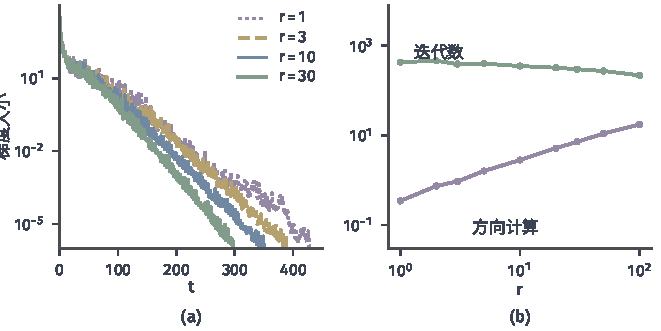
\includegraphics[width=112mm]{figures/05-optimization/02-smooth-optimization/matplotlib/qn-lbfgs-memory/figure.pdf}
  \caption{记忆长度的影响。目标是$200$维的$\sum_i(\tfrac12c_iz_i^2+\ln\cosh z_i)$，$\bm{z}=\bm{Q}\bm{x}$，$\bm{Q}$是固定的正交矩阵，$c_i$在$[10^{-3},10^{3}]$上对数等距，强Wolfe线搜索，$c_2=0.9$。(a)不同$r$下的梯度大小。(b)达到梯度大小$10^{-6}$的迭代数（绿）和这些迭代中方向计算的总乘法次数（紫，单位百万次，按每步$4rn$估算）。}
  \label{fig:qn-lbfgs-memory}
\end{BookInlineFigure}

\paragraph{初始缩放的影响}
图~\ref{fig:qn-lbfgs-scaling}比较有缩放~\eqref{eq:qn-lbfgs-gamma}和始终用$\gamma=1$的两种做法，记忆长度都是$r=10$，目标的曲率整体偏大。

没有缩放时，单位矩阵相对于真实曲率过大，方向过长，线搜索不得不反复收缩，$292$轮迭代共用了$5012$次函数和梯度计算。有缩放时只用$130$轮迭代和$268$次计算。这个对比说明，在大尺度问题上，第~\ref{sec:qn-secant}节“优先试单位步长”的策略依赖矩阵有正确的尺度。

\begin{BookInlineFigure}
  \centering
  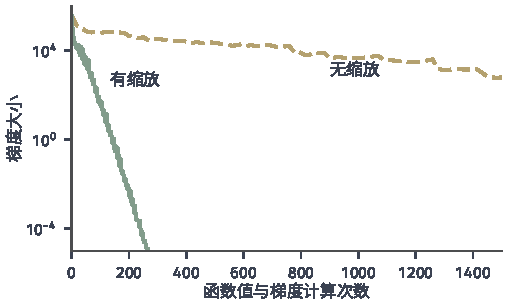
\includegraphics[width=86mm]{figures/05-optimization/02-smooth-optimization/matplotlib/qn-lbfgs-scaling/figure.pdf}
  \caption{初始缩放的影响：$r=10$，目标是$n=200$的旋转$\ln\cosh$函数（$c_i$在$[0.01,100]$上对数等距）再乘以$1000$，强Wolfe线搜索。绿线取式~\eqref{eq:qn-lbfgs-gamma}的缩放，黄虚线始终取$\gamma=1$。横轴是函数值与梯度的计算次数，纵轴是梯度大小。}
  \label{fig:qn-lbfgs-scaling}
\end{BookInlineFigure}

\section{收敛与计算成本}
\label{sec:qn-convergence}

前面各节展示了许多好现象，但例子都很小。于是要问：这些方法在什么条件下能保证什么？答案要分开说，因为不同的更新规则、线搜索和目标类型，对应的结论强弱不同。

全节的基本假设是：$f$二阶连续可微，存在$0<\mu\leq L$使$\mu\bm{I}\preceq\nabla^2f(\bm{x})\preceq L\bm{I}$对所有$\bm{x}$成立，$\bm{x}^\star$是唯一最优解。需要放宽时会明确说明。

\paragraph{一步下降与方向角}
先把线搜索的贡献算清楚。记$\theta^{(t)}$为$\bm{d}^{(t)}$与$-\bm{g}^{(t)}$的夹角，
\begin{equation}
 \cos\theta^{(t)}=\frac{-\langle\bm{g}^{(t)},\bm{d}^{(t)}\rangle}{\lVert\bm{g}^{(t)}\rVert_2\lVert\bm{d}^{(t)}\rVert_2}.
 \label{eq:qn-cos-theta}
\end{equation}
方向越接近负梯度，$\cos\theta^{(t)}$越接近$1$；方向几乎与梯度垂直时，它接近$0$，再好的步长也下降有限。

\begin{lemma}[Wolfe线搜索的一步下降]
\label{lem:qn-one-step}
设$\nabla f$是$L$-Lipschitz的，$\bm{d}^{(t)}$是下降方向，$\alpha^{(t)}$满足式~\eqref{eq:qn-wolfe}。则
\begin{equation}
 f(\bm{x}^{(t+1)})\leq f(\bm{x}^{(t)})-\frac{c_1(1-c_2)}{L}\cos^2\theta^{(t)}\lVert\bm{g}^{(t)}\rVert_2^2.
 \label{eq:qn-one-step}
\end{equation}
\end{lemma}

\begin{proof}
省略上标。由第二条Wolfe不等式和梯度的Lipschitz性，得到
\[
 (c_2-1)\langle\bm{g},\bm{d}\rangle\leq\langle\bm{g}^{+}-\bm{g},\bm{d}\rangle\leq\alpha L\lVert\bm{d}\rVert_2^2.
\]

这给出步长的下界：
\[
 \alpha\geq\frac{(1-c_2)\lvert\langle\bm{g},\bm{d}\rangle\rvert}{L\lVert\bm{d}\rVert_2^2}.
\]

把它代入第一条Wolfe不等式，并用式~\eqref{eq:qn-cos-theta}，得到
\[
 f(\bm{x}^{+})\leq f(\bm{x})-c_1\alpha\lvert\langle\bm{g},\bm{d}\rangle\rvert
 \leq f(\bm{x})-\frac{c_1(1-c_2)}{L}\cdot\frac{\langle\bm{g},\bm{d}\rangle^2}{\lVert\bm{d}\rVert_2^2},
\]
最后一个分式等于$\cos^2\theta\lVert\bm{g}\rVert_2^2$。
\end{proof}

把式~\eqref{eq:qn-one-step}对$t$求和，并用$f$有下界，就得到称为\term{Zoutendijk条件}（Zoutendijk condition）的结论$\sum_t\cos^2\theta^{(t)}\lVert\bm{g}^{(t)}\rVert_2^2<\infty$。所以只要$\cos\theta^{(t)}$不趋于零，梯度就要趋于零。全局收敛的问题变成：方向角能不能控制住？

\paragraph{BFGS的全局收敛}
BFGS的矩阵可能很差，方向可能很偏。下面的定理说，只要目标强凸，差的方向不可能一直出现。证明的工具是一个衡量矩阵“病态程度”的势函数，这也就是自校正的数学内容。

\begin{theorem}[BFGS在强凸目标上的全局收敛]
\label{thm:qn-bfgs-global}
设$f$满足本节的基本假设，$\bm{B}^{(0)}\succ\bm{0}$，步长满足Wolfe条件~\eqref{eq:qn-wolfe}，所有$\bm{g}^{(t)}\neq\bm{0}$。则BFGS的迭代点满足
\begin{equation}
 \lim_{t\to\infty}\bm{x}^{(t)}=\bm{x}^\star.
 \label{eq:qn-bfgs-global}
\end{equation}
\end{theorem}

\begin{proof}
由式~\eqref{eq:qn-wolfe-curvature}和定理~\ref{thm:qn-positive-definite}，所有$\bm{B}^{(t)}$正定。定义势函数
\[
 \psi(\bm{B})=\operatorname{tr}\bm{B}-\ln\det\bm{B}=\sum_{i=1}^n(\lambda_i-\ln\lambda_i),
\]
其中$\lambda_i$是$\bm{B}$的特征值。因为$\lambda-\ln\lambda\geq1$，所以$\psi(\bm{B})>0$。它同时惩罚过大和过小的特征值。

第一步，估计测量的尺度。省略上标，由式~\eqref{eq:qn-average-hessian}，并令$\bm{z}=\bar{\bm{H}}^{1/2}\bm{s}$，得到
\[
 \frac{\langle\bm{s},\bm{y}\rangle}{\langle\bm{s},\bm{s}\rangle}\geq\mu,\qquad
 \frac{\langle\bm{y},\bm{y}\rangle}{\langle\bm{s},\bm{y}\rangle}=\frac{\bm{z}^\top\bar{\bm{H}}\bm{z}}{\bm{z}^\top\bm{z}}\leq L.
\]

第二步，计算迹和行列式的变化。对式~\eqref{eq:qn-bfgs-direct}取迹，得到
\[
 \operatorname{tr}\bm{B}^{+}=\operatorname{tr}\bm{B}-\frac{\lVert\bm{B}\bm{s}\rVert_2^2}{\bm{s}^\top\bm{B}\bm{s}}+\frac{\lVert\bm{y}\rVert_2^2}{\langle\bm{s},\bm{y}\rangle}.
\]

行列式把$\bm{B}$提出来，写成
\[
 \det\bm{B}^{+}=\det\bm{B}\cdot\det\Bigl(\bm{I}-\frac{\bm{s}(\bm{B}\bm{s})^\top}{\bm{s}^\top\bm{B}\bm{s}}+\rho\,\bm{W}\bm{y}\bm{y}^\top\Bigr).
\]
括号内是$\bm{I}+\bm{U}\bm{C}^\top$的形式，其中$\bm{U}$的两列是$-\bm{s}/(\bm{s}^\top\bm{B}\bm{s})$与$\rho\bm{W}\bm{y}$，$\bm{C}$的两列是$\bm{B}\bm{s}$与$\bm{y}$。由行列式的恒等式（交换乘积因子，维数从$n$降到$2$），$\bm{I}+\bm{U}\bm{C}^\top$与$\bm{I}+\bm{C}^\top\bm{U}$的行列式相同。沿用第~\ref{sec:qn-dfp-bfgs}节的曲率比$\tau$，则
\[
 \bm{I}+\bm{C}^\top\bm{U}=\begin{bmatrix}0&1\\-\tau&1+\rho\,\bm{y}^\top\bm{W}\bm{y}\end{bmatrix},
\]
这个矩阵的行列式是$\tau$，因此
\[
 \det\bm{B}^{+}=\det\bm{B}\cdot\frac{\langle\bm{s},\bm{y}\rangle}{\bm{s}^\top\bm{B}\bm{s}}.
\]

第三步，用方向角重写。由$\bm{B}\bm{d}=-\bm{g}$和$\bm{s}=\alpha\bm{d}$，式~\eqref{eq:qn-cos-theta}的夹角满足
\[
 \cos\theta=\frac{\bm{s}^\top\bm{B}\bm{s}}{\lVert\bm{s}\rVert_2\lVert\bm{B}\bm{s}\rVert_2}.
\]

再引入三个比值：
\[
 q=\frac{\bm{s}^\top\bm{B}\bm{s}}{\langle\bm{s},\bm{s}\rangle},\qquad m_{\mathrm{c}}=\frac{\langle\bm{s},\bm{y}\rangle}{\langle\bm{s},\bm{s}\rangle},\qquad M_{\mathrm{c}}=\frac{\langle\bm{y},\bm{y}\rangle}{\langle\bm{s},\bm{y}\rangle}.
\]
于是迹和行列式公式中的两个量可以写成
\[
 \frac{\lVert\bm{B}\bm{s}\rVert_2^2}{\bm{s}^\top\bm{B}\bm{s}}=\frac{q}{\cos^2\theta},\qquad
 \frac{\langle\bm{s},\bm{y}\rangle}{\bm{s}^\top\bm{B}\bm{s}}=\frac{m_{\mathrm{c}}}{q}.
\]

把第二步的结果代入$\psi$，整理得到
\[
 \psi(\bm{B}^{+})=\psi(\bm{B})+(M_{\mathrm{c}}-\ln m_{\mathrm{c}}-1)
 +\Bigl[1-\frac{q}{\cos^2\theta}+\ln\frac{q}{\cos^2\theta}\Bigr]+\ln\cos^2\theta.
\]
方括号非正，因为$1-v+\ln v\leq0$对$v>0$成立。令$c=\max\{L-\ln\mu-1,\,1\}>0$，由第一步，
\[
 \psi(\bm{B}^{(t+1)})\leq\psi(\bm{B}^{(0)})+c(t+1)+\sum_{j=0}^{t}\ln\cos^2\theta^{(j)}.
\]

第四步，反证。设$\cos\theta^{(t)}\to0$，则存在$t_1$，当$j>t_1$时$\ln\cos^2\theta^{(j)}<-2c$。对$t>t_1$，上式右端不超过
\[
 \psi(\bm{B}^{(0)})+c(t+1)+\sum_{j\leq t_1}\ln\cos^2\theta^{(j)}-2c(t-t_1).
\]
它随$t$线性趋于$-\infty$，与$\psi>0$矛盾。所以存在$\delta>0$和子列使$\cos\theta^{(t)}\geq\delta$。

第五步，收敛。对引理~\ref{lem:qn-one-step}求和，得到Zoutendijk条件，所以沿这个子列$\lVert\bm{g}^{(t)}\rVert_2\to0$。第~\ref{chap:optimization}章的误差换算给出下面两个不等式：
\[
 f(\bm{x})-f^\star\leq\frac{\lVert\nabla f(\bm{x})\rVert_2^2}{2\mu},\qquad
 \frac{\mu}{2}\lVert\bm{x}-\bm{x}^\star\rVert_2^2\leq f(\bm{x})-f^\star.
\]
前一个说明沿子列$f(\bm{x}^{(t)})\to f^\star$。

$f(\bm{x}^{(t)})$单调，于是整个序列的目标值都收敛到$f^\star$。再由后一个不等式，迭代点收敛到$\bm{x}^\star$。
\end{proof}

用贯穿例的BFGS（$\bm{B}^{(0)}=\bm{I}$，精确线搜索）核对一下这个公式。三个矩阵的$\psi$值是
\[
 \begin{gathered}
 \psi(\bm{B}^{(0)})=2,\qquad\psi(\bm{B}^{(1)})=7.8-\ln5\approx6.191,\\
 \psi(\bm{B}^{(2)})=10-\ln16\approx7.227.
 \end{gathered}
\]

第一次更新$\cos\theta^{(0)}=1$、$q=1$，方括号与最后的对数都是零，增量全部来自尺度项。按定理证明中的记号，$M_{\mathrm{c}}=6.8$，$m_{\mathrm{c}}=5$，于是
\[
 \psi(\bm{B}^{(1)})-\psi(\bm{B}^{(0)})=6.8-\ln5-1\approx4.191.
\]

第二次更新的方向角满足$\cos^2\theta^{(1)}\approx0.735$，此时$q/\cos^2\theta^{(1)}=1$，方括号仍是零。尺度项是$3.2-\ln2.353-1\approx1.344$，而$\ln\cos^2\theta^{(1)}\approx-0.308$，两者之和与$\psi$的实际增量$1.036$一致。

定理的证明解释了自校正：$\psi$每一步至多增加一个常数，而每次方向偏得厉害都要付出$\ln\cos^2\theta$这一项的大幅减少，方向不可能一直偏。证明中的第二步用到了BFGS特有的迹和行列式公式，不能搬给DFP；我们也不声称DFP在Wolfe线搜索下有同样的结论，图~\ref{fig:qn-dfp-bfgs-scaling}(b)显示它确实可能很慢。

对一般非凸目标，没有类似的定理：已有构造性例子说明，即使线搜索满足Wolfe条件，BFGS也可能不收敛到驻点。实践中BFGS常常工作良好，但这不是定理所保证的。

\paragraph{局部收敛的刻画：Dennis--Moré条件}
全局收敛说的是终将到达，还要看到达的速度。称$\bm{x}^{(t)}\to\bm{x}^\star$是\term{超线性收敛}（superlinear convergence），如果
\begin{equation}
 \lim_{t\to\infty}\frac{\lVert\bm{x}^{(t+1)}-\bm{x}^\star\rVert_2}{\lVert\bm{x}^{(t)}-\bm{x}^\star\rVert_2}=0.
 \label{eq:qn-superlinear}
\end{equation}
Newton法靠的是矩阵趋于Hessian。拟牛顿矩阵一般并不趋于Hessian，超线性收敛却仍然可能发生。下面的定理说明，真正需要的只是沿步方向准确。

\begin{theorem}[Dennis--Moré特征]
\label{thm:qn-dennis-more}
设$f$二阶连续可微，$\bm{x}^{(t)}\to\bm{x}^\star$，$\bm{x}^\star$是驻点，$\bm{H}^\star=\nabla^2f(\bm{x}^\star)$正定。设对充分大的$t$，迭代取单位步长且方向$\bm{d}^{(t)}\neq\bm{0}$由$\bm{B}^{(t)}\bm{d}^{(t)}=-\bm{g}^{(t)}$确定。则序列超线性收敛，当且仅当
\begin{equation}
 \lim_{t\to\infty}\frac{\lVert(\bm{B}^{(t)}-\bm{H}^\star)\bm{d}^{(t)}\rVert_2}{\lVert\bm{d}^{(t)}\rVert_2}=0.
 \label{eq:qn-dennis-more}
\end{equation}
\end{theorem}

\begin{proof}
省略上标，把误差写成$\bm{e}=\bm{x}-\bm{x}^\star$、$\bm{e}^{+}=\bm{x}^{+}-\bm{x}^\star$。与式~\eqref{eq:qn-average-hessian}一样，梯度差等于平均Hessian乘$\bm{d}$。代入$\bm{g}=-\bm{B}\bm{d}$，得到关键等式
\[
 \bm{g}^{+}=(\bar{\bm{H}}-\bm{H}^\star)\bm{d}+(\bm{H}^\star-\bm{B})\bm{d}.
\]
因为$\bm{x}^{(t)}\to\bm{x}^\star$且Hessian连续，所以$\bar{\bm{H}}\to\bm{H}^\star$，第一项是$o(\lVert\bm{d}\rVert_2)$。

充分性：设式~\eqref{eq:qn-dennis-more}成立，则$\lVert\bm{g}^{+}\rVert_2=o(\lVert\bm{d}\rVert_2)$。在$\bm{x}^\star$附近，$\nabla^2f$的最小特征值不小于某个$\mu_{\star}>0$，所以
\[
 \lVert\bm{g}^{+}\rVert_2\geq\mu_{\star}\lVert\bm{e}^{+}\rVert_2.
\]

再由三角不等式，$\lVert\bm{d}\rVert_2$不超过两个误差的范数之和，于是
\[
 \lVert\bm{e}^{+}\rVert_2\leq o(1)\bigl(\lVert\bm{e}\rVert_2+\lVert\bm{e}^{+}\rVert_2\bigr).
\]
移项即得$\lVert\bm{e}^{+}\rVert_2=o(\lVert\bm{e}\rVert_2)$。

必要性：设序列超线性收敛。由三角不等式，$\lVert\bm{d}\rVert_2$不小于$\lVert\bm{e}\rVert_2-\lVert\bm{e}^{+}\rVert_2$，而$\lVert\bm{e}^{+}\rVert_2=o(\lVert\bm{e}\rVert_2)$，于是$\lVert\bm{e}\rVert_2=O(\lVert\bm{d}\rVert_2)$。

$\nabla f$在$\bm{x}^\star$处为零且连续可微，所以$\lVert\bm{g}^{+}\rVert_2$是$\lVert\bm{e}^{+}\rVert_2$的同阶小量，于是
\[
 \lVert\bm{g}^{+}\rVert_2=o(\lVert\bm{e}\rVert_2)=o(\lVert\bm{d}\rVert_2).
\]
由关键等式解出第二项，并用$\bar{\bm{H}}\to\bm{H}^\star$，得到式~\eqref{eq:qn-dennis-more}。
\end{proof}

式~\eqref{eq:qn-dennis-more}称为\term{Dennis--Moré条件}（Dennis--Moré condition）。它只比较矩阵在搜索方向上的作用，所以拟牛顿矩阵不必收敛到Hessian。图~\ref{fig:qn-rates}(b)印证了这一点：迭代结束时矩阵整体的误差约为$3\%$，沿步方向的误差约为$0.08\%$。

定理假设步长最终是$1$。满足式~\eqref{eq:qn-dennis-more}且$c_1<1/2$时，Wolfe线搜索最终确实接受单位步长，证明可查阅\scite{math-nocedal2006numerical}。这也是线搜索要优先试$\alpha=1$的理由：如果不试，或者试了又不接受，上面的超线性机制就用不上。

\paragraph{BFGS的超线性收敛}
完整记忆的BFGS确实满足Dennis--Moré条件，但需要更强的正则性。若$\bm{x}^{(t)}\to\bm{x}^\star$，$\bm{H}^\star$正定，$\nabla^2f$在$\bm{x}^\star$附近Lipschitz连续，且$\sum_t\lVert\bm{x}^{(t)}-\bm{x}^\star\rVert_2<\infty$，又有单位步长优先试探的线搜索，则BFGS超线性收敛。

证明要沿用定理~\ref{thm:qn-bfgs-global}的势函数并在$\bm{H}^\star$定义的坐标下估计，篇幅较长，读者可查阅\scite{math-nocedal2006numerical}。求和条件要求误差足够快地衰减，在定理~\ref{thm:qn-bfgs-global}的强凸条件下可以进一步证明它成立。Lipschitz条件的作用是控制$\bar{\bm{H}}^{(t)}$与$\bm{H}^\star$之差，使测量误差可以累加。

\begin{BookInlineFigure}
  \centering
  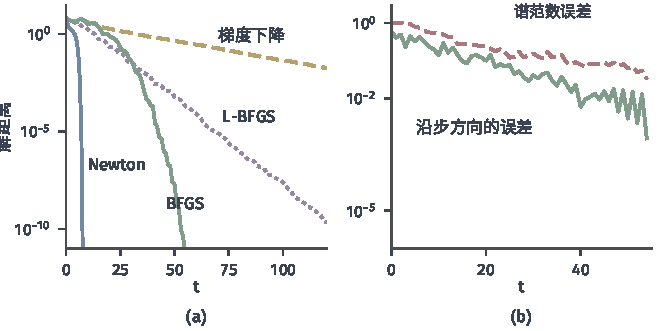
\includegraphics[width=112mm]{figures/05-optimization/02-smooth-optimization/matplotlib/qn-rates/figure.pdf}
  \caption{不同方法的局部速度，目标是$50$维的旋转$\ln\cosh$函数（$c_i$在$[0.1,100]$上对数等距，$\bm{x}^\star=\bm{0}$），强Wolfe线搜索。(a)解距离随迭代的变化：梯度下降（黄虚线）线性且慢，$r=5$的L-BFGS（紫点线）线性，BFGS（绿）后期斜率变陡，Newton法（蓝）最快。(b)BFGS的矩阵相对误差：红虚线是$\lVert\bm{B}^{(t)}-\bm{H}^\star\rVert_2/\lVert\bm{H}^\star\rVert_2$，绿线是Dennis--Moré比值$\lVert(\bm{B}^{(t)}-\bm{H}^\star)\bm{s}^{(t)}\rVert_2/(\lVert\bm{H}^\star\rVert_2\lVert\bm{s}^{(t)}\rVert_2)$。}
  \label{fig:qn-rates}
\end{BookInlineFigure}

\paragraph{SR1的局部结论}
SR1的结论需要不同的条件，第~\ref{sec:qn-sr1}节的定理只覆盖二次目标。对一般目标，已有的结果大致是：在$\bm{H}^\star$正定、分母保持远离零、步方向具有一致线性无关性质时，$\bm{B}^{(t)}$本身收敛到Hessian，配合信赖域可得到$n+1$步意义下的超线性收敛。这些条件比BFGS的条件更难事先验证，也不能换成Wolfe线搜索下的方向分析；相应证明见\scite{math-nocedal2006numerical}。

\paragraph{L-BFGS只保证线性收敛}
完整BFGS的超线性结论不能自动移给固定记忆的L-BFGS。超线性机制要求矩阵逐渐掌握沿步方向的曲率，而每轮重新从$\gamma\bm{I}$开始、只用$r$对向量的矩阵，无法累积足够的信息。下面的定理给出固定记忆下能证明的保证。

\begin{theorem}[L-BFGS的线性收敛]
\label{thm:qn-lbfgs-linear}
设$f$满足本节的基本假设，$t\geq1$时$\gamma^{(t)}$由式~\eqref{eq:qn-lbfgs-gamma}给出，$t=0$时取负梯度方向，记忆长度为$r$，步长满足Wolfe条件。令$T_{\mathrm{c}}=(n+r)L$，$\delta=(\mu/T_{\mathrm{c}})^{n+r}$。则
\begin{equation}
 f(\bm{x}^{(t+1)})-f^\star\leq\Bigl(1-\frac{2\mu c_1(1-c_2)\delta^2}{L}\Bigr)\bigl(f(\bm{x}^{(t)})-f^\star\bigr).
 \label{eq:qn-lbfgs-linear}
\end{equation}
\end{theorem}

\begin{proof}
设$\bm{B}_{[j]}=\bm{W}_{[j]}^{-1}$，它们由$\bm{B}_{[t-r]}=(1/\gamma^{(t)})\bm{I}$出发，按BFGS的直接形式更新$r$次。第一步，由定理~\ref{thm:qn-bfgs-global}证明中的尺度估计，$1/\gamma^{(t)}\in[\mu,L]$。

第二步，约束迹。式~\eqref{eq:qn-bfgs-direct}的修正中，减去的一项迹非负，加上的一项迹不超过$L$，于是
\[
 \operatorname{tr}\bm{B}_{[t]}\leq\frac{n}{\gamma^{(t)}}+rL\leq(n+r)L=T_{\mathrm{c}}.
\]
所以每个$\bm{B}_{[j]}$的最大特征值不超过$T_{\mathrm{c}}$。

第三步，约束行列式。由行列式公式和第一步，每次更新满足
\[
 \frac{\det\bm{B}_{[j+1]}}{\det\bm{B}_{[j]}}=\frac{\langle\bm{s},\bm{y}\rangle}{\bm{s}^\top\bm{B}_{[j]}\bm{s}}\geq\frac{\mu\lVert\bm{s}\rVert_2^2}{T_{\mathrm{c}}\lVert\bm{s}\rVert_2^2}=\frac{\mu}{T_{\mathrm{c}}}.
\]
连乘至多$r$次（窗口未满时次数更少，因$\mu/T_{\mathrm{c}}\leq1$，下界不变），并用$\det\bm{B}_{[t-r]}\geq\mu^n$，得到
\[
 \det\bm{B}^{(t)}\geq\mu^n\Bigl(\frac{\mu}{T_{\mathrm{c}}}\Bigr)^r.
\]

第四步，约束方向角。最小特征值至少是行列式除以另外$n-1$个特征值的上界，所以$\bm{B}^{(t)}$的条件数不超过
\[
 \frac{T_{\mathrm{c}}^{\,n}}{\det\bm{B}^{(t)}}\leq\Bigl(\frac{T_{\mathrm{c}}}{\mu}\Bigr)^{n+r}=\frac{1}{\delta}.
\]

由$\bm{d}=-\bm{W}\bm{g}$，方向角满足
\[
 \cos\theta^{(t)}=\frac{\bm{g}^\top\bm{W}\bm{g}}{\lVert\bm{g}\rVert_2\lVert\bm{W}\bm{g}\rVert_2}\geq\frac{\lambda_{\min}(\bm{W})}{\lambda_{\max}(\bm{W})}\geq\delta.
\]

第五步，代入引理~\ref{lem:qn-one-step}，并用第~\ref{chap:optimization}章的$\lVert\bm{g}\rVert_2^2\geq2\mu(f-f^\star)$，即得式~\eqref{eq:qn-lbfgs-linear}。
\end{proof}

定理的常数$\delta$随$n+r$指数变小，几乎没有定量价值。它的意义在于定性：固定记忆时，矩阵的条件数有界，因而线性收敛，且这个结论不依赖超线性的机制。图~\ref{fig:qn-rates}(a)中L-BFGS的直线正是线性收敛的样子，实际的速度远比定理的常数好。

\paragraph{各方法的保证}
下表汇总本节的结论，列出的是使结论成立的条件，并非全部的可行条件。

\begin{BookInlineTable}
  \centering
  \small
  \begin{tabular}{p{15mm}p{39mm}p{39mm}}
    \toprule
    方法 & 全局 & 局部\\
    \midrule
    BFGS & 强凸＋Wolfe：收敛（已证） & Hessian Lipschitz、误差可和：超线性\\
    DFP & 本章的势函数论证不适用 & 不作结论\\
    SR1 & 二次目标：至多$n+1$步（已证） & 分母与步方向条件＋信赖域：$n+1$步意义下超线性\\
    L-BFGS & 强凸＋Wolfe：线性收敛（已证） & 不保证超线性\\
    \bottomrule
  \end{tabular}
  \caption{拟牛顿方法的收敛保证汇总。}
  \label{tab:qn-guarantees}
\end{BookInlineTable}

\paragraph{计算成本}
比较成本要固定相同的精度，并把各项都算上。下表列出每一步除梯度外的开销，$n$是变量维数，$r$是记忆长度，线搜索的函数和梯度计算次数另算。

\begin{BookInlineTable}
  \centering
  \begin{tabular}{lll}
    \toprule
    方法 & 存储 & 方向与更新的乘法次数\\
    \midrule
    梯度下降 & $n$ & $n$\\
    L-BFGS & $2rn$ & $(4r+1)n$\\
    BFGS、DFP、SR1 & $n^2/2$ & 约$4n^2$\\
    Newton法 & $n^2/2$ & 约$n^3/3$，另加形成Hessian\\
    \bottomrule
  \end{tabular}
  \caption{每步除梯度以外的存储与运算，Newton法按Cholesky分解计。}
  \label{tab:qn-cost}
\end{BookInlineTable}

单步开销低的方法不一定总开销低，要乘上迭代数才能比较。图~\ref{fig:qn-rates}的目标取$n=50$，达到解距离$10^{-8}$需要的迭代数和方向运算量如表~\ref{tab:qn-experiment-cost}所示。

\begin{BookInlineTable}
  \centering
  \begin{tabular}{lrrr}
    \toprule
    方法 & 迭代数 & 每步方向运算 & 方向运算合计\\
    \midrule
    梯度下降 & $458$ & $50$ & $2.3\times10^{4}$\\
    L-BFGS（$r=5$） & $104$ & $1050$ & $1.1\times10^{5}$\\
    BFGS & $51$ & $1.0\times10^{4}$ & $5.1\times10^{5}$\\
    Newton法 & $8$ & $4.2\times10^{4}$ & $3.3\times10^{5}$\\
    \bottomrule
  \end{tabular}
  \caption{图~\ref{fig:qn-rates}的目标（$n=50$）上达到解距离$10^{-8}$的迭代数与方向运算量，不含梯度和Hessian的计算。}
  \label{tab:qn-experiment-cost}
\end{BookInlineTable}

这张表不能单独读。这个目标上一次梯度要做两次$50\times50$的矩阵乘法，约$5000$次运算，所以梯度下降实际花在梯度上的开销约为$2.3\times10^{6}$，远超方向运算本身。Newton法的Hessian开销未计入；在$n=50$时分解很便宜，$n$增大后三次方项才成为主要矛盾。比较的结论要在实际的$n$、梯度和Hessian成本下重新算。

实际选择大致如下：$n$不大、梯度贵、要高精度时用完整BFGS；$n$很大时用L-BFGS，代价是只有线性速度的保证；需要负曲率信息时用SR1配信赖域。

\section{本章小结}
\label{sec:qn-summary}

本章开头的问题是：Hessian算不起、存不下时，能否从迭代本身得到曲率信息。答案是相邻两点的梯度差。式~\eqref{eq:qn-average-hessian}说明它是平均Hessian作用在位移上的结果，由此得到割线条件。这个条件在$n=1$时确定了曲率，$n>1$时还缺$n(n-1)/2$个方程，所以需要补充对称、低秩和曲率的要求。

不同的补充要求产生了不同的方法。DFP和BFGS各用两个秩一项，分别在矩阵和逆矩阵上度量改动。两者都在曲率条件$\langle\bm{s},\bm{y}\rangle>0$下保持正定，Wolfe线搜索使这个条件对任意光滑目标成立，跳过和阻尼是线搜索之外的备用办法。

SR1只用一个秩一项，由割线条件唯一确定。它在二次目标上有更强的遗传性质，能记录负曲率，但分母可能近零，矩阵也可能不定，所以需要跳过规则，且方向分析不能照搬，要交给有界的模型处理。

L-BFGS用双循环递推在不保存矩阵的情况下计算$\bm{W}^{(t)}\bm{g}^{(t)}$，把存储从$n^2/2$降到$2rn$。记忆长度决定了方向的质量和每步的计算量，初始缩放决定了单位步长是否合适。

\begin{BookInlineTable}
  \centering
  \begin{tabular}{llll}
    \toprule
    方法 & 新增信息 & 保持的性质 & 单步主要开销\\
    \midrule
    BFGS & 秩二修正 & 曲率条件下正定 & $O(n^2)$\\
    DFP & 秩二修正 & 曲率条件下正定 & $O(n^2)$\\
    SR1 & 秩一修正 & 可表示负曲率 & $O(n^2)$\\
    L-BFGS & 最近$r$对 & 曲率条件下正定 & $O(rn)$\\
    \bottomrule
  \end{tabular}
  \caption{本章四种拟牛顿方法的比较。}
  \label{tab:qn-summary}
\end{BookInlineTable}

收敛结论要分开看。BFGS在强凸目标和Wolfe线搜索下全局收敛，在更强的正则性下超线性收敛，后者由Dennis--Mor\'e条件刻画，它只要求沿步方向准确。L-BFGS在强凸目标上线性收敛，完整记忆的超线性结论不能自动移给它。一般非凸目标上，这些保证都不成立，SR1在一般目标上的局部结论也有额外条件。

拟牛顿矩阵的好坏，最终还要看模型在多大范围内可信。线搜索只沿一个方向试探，不定模型又没有极小点；第~\ref{chap:trust-region}章研究的信赖域，把候选步和接受判断放在一起处理，并且既可以用精确Hessian，也可以用本章的拟牛顿矩阵。

